\documentclass[14pt]{mmcs_article}
\usepackage[russian]{babel}
\usepackage{amsmath, amsthm, amsfonts, amssymb}
\geometry{left=3cm,right=1.5cm,top=2cm,bottom=2cm}
\setlength{\parindent}{1.25cm}

\graphicspath{{images/}}%путь к рисункам
\usepackage[usenames]{color}
\usepackage{colortbl}

\begin{document}

% Титульные листы
% раскомментировать требуемое
%%см. РЕКОМЕНДАЦИИ ПО ОФОРМЛЕНИЮ
%И ПРЕДСТАВЛЕНИЮ КУРСОВЫХ И ВЫПУСКНЫХ %КВАЛИФИКАЦИОННЫХ РАБОТ СТУДЕНТОВ ИНСТИТУТА %МАТЕМАТИКИ, МЕХАНИКИ И КОМПЬЮТЕРНЫХ НАУК


% ----------------------------------
% Внимание!
% Изменяйте только строки, перед которыми стоят знаки комментариев
% ----------------------------------

\thispagestyle{empty}
\begin{singlespacing}
\begin{center}

МИНОБРНАУКИ РОССИИ\\ [12pt]
Федеральное государственное автономное образовательное\\
учреждение высшего образования\\
<<Южный федеральный университет>>

\vspace{\baselineskip}
Институт математики, механики\\
и компьютерных наук им.~И.\,И.~Воровича

\vspace{\baselineskip}
% Название выпускающей кафедры
Кафедра алгебры и дискретной математики

\vfill
% Фамилия Имя Отчество студента
\textbf{Иванов Сергей Иванович}

\vspace{\baselineskip}
%%НАЗВАНИЕ РАБОТЫ должно полностью соответствовать распоряжению по Институту (для курсовых работ).
{\bf НАЗВАНИЕ РАБОТЫ, \\
РАЗБИТОЕ ПРИ НЕОБХОДИМОСТИ \\
НА НЕСКОЛЬКО СТРОК }

\vspace{15mm}
КУРСОВАЯ РАБОТА\\
по направлению подготовки\\
% указать направление обучения (раскомментируйте нужную строчку)
01.03.02~-- Прикладная математика и информатика
% 01.03.01~-- Математика
% 01.03.03~-- Механика и математическое моделирование 	
% 02.03.02~-- Фундаментальная информатика и информационные технологии


\vspace{10mm}
\textbf{Научный руководитель~--}\\
% указать данные о руководителе
% должность, степень, звание Фамилия Имя Отчество
проф., д.\,ф.-м.\,н. Сергеев Петр Сергеевич

\vspace{20mm}

\noindent
\begin{flushleft}
$\overline{\textrm{оценка (рейтинг)}}$\qquad	$\overline{\textrm{подпись руководителя\vphantom{й}}}$

\end{flushleft}


\vfill
% год!
Ростов-на-Дону -- 2020

\end{center}

\singlespacing
\end{singlespacing}  % для курсовой
%см. РЕКОМЕНДАЦИИ ПО ОФОРМЛЕНИЮ
%И ПРЕДСТАВЛЕНИЮ КУРСОВЫХ И ВЫПУСКНЫХ %КВАЛИФИКАЦИОННЫХ РАБОТ СТУДЕНТОВ ИНСТИТУТА %МАТЕМАТИКИ, МЕХАНИКИ И КОМПЬЮТЕРНЫХ НАУК


% ----------------------------------
% Внимание!
% Изменяйте только строки, перед которыми стоят знаки комментариев
% ----------------------------------

\thispagestyle{empty}
\begin{singlespacing}
\begin{center}

МИНОБРНАУКИ РОССИИ\\ [12pt]
Федеральное государственное автономное образовательное\\
учреждение высшего образования\\
<<Южный федеральный университет>>

\vspace{\baselineskip}
Институт математики, механики\\
и компьютерных наук им.~И.\,И.~Воровича

\vspace{\baselineskip}
% Название выпускающей кафедры
Кафедра информатики и вычислительного эксперимента

\vfill
% Фамилия Имя Отчество студента
\textbf{Волнобой Ирина Леонидовна}

\vspace{\baselineskip}
%НАЗВАНИЕ РАБОТЫ должно полностью соответствовать
% приказу по ЮФУ (для выпускных квалификационных работ)
{\bf РАЗРАБОТКА КОМПОНЕНТОВ ПРИЛОЖЕНИЯ \\
ДЛЯ АНАЛИЗА ОНЛАЙН-ПРОФИЛЯ \\
ЖИВОТНОГО ИЗ ПРИЮТА }


\vspace{15mm}
ВЫПУСКНАЯ КВАЛИФИКАЦИОННАЯ РАБОТА\\
по направлению подготовки\\
% Направление обучения
% раскомментируйте нужную строчку
02.03.02~-- Фундаментальная информатика и информационные технологии
% 01.03.01~-- Математика
% 01.03.02~-- Прикладная математика и информатика
% 01.03.03~-- Механика и математическое моделирование 	


\vspace{10mm}
\textbf{Научный руководитель~--}\\
% указать данные о руководителе
% должность, степень, звание Фамилия Имя Отчество 
доцент., к.\,ф.-м.\,н. Абрамян Анна Владимировна

\vspace{15mm}

\noindent
% указать Фамилию и инициалы 
% заведующего выпускающей кафедры
\begin{flushleft}
Допущено к защите:\\
заведующий кафедрой \underline{\hspace*{65mm}} Михалкович С.\,С.
\end{flushleft}




\vfill
% год!
Ростов-на-Дону -- 2021

\end{center}

\singlespacing
\end{singlespacing} % для работы бакалавра
%%см. РЕКОМЕНДАЦИИ ПО ОФОРМЛЕНИЮ
%И ПРЕДСТАВЛЕНИЮ КУРСОВЫХ И ВЫПУСКНЫХ %КВАЛИФИКАЦИОННЫХ РАБОТ СТУДЕНТОВ ИНСТИТУТА %МАТЕМАТИКИ, МЕХАНИКИ И КОМПЬЮТЕРНЫХ НАУК


% ----------------------------------
% Внимание!
% Изменяйте только строки, перед которыми стоят знаки комментариев
% ----------------------------------

\thispagestyle{empty}
\begin{singlespacing} 
\begin{center}

МИНОБРНАУКИ РОССИИ\\ [12pt]
Федеральное государственное автономное образовательное\\
учреждение высшего образования\\
<<Южный федеральный университет>>

\vspace{\baselineskip}
Институт математики, механики\\
и компьютерных наук им.~И.\,И.~Воровича


\vfill
% Фамилия Имя Отчество студента
\textbf{Иванов Сергей Иванович}

\vspace{15mm}
%НАЗВАНИЕ РАБОТЫ должно полностью соответствовать 
% приказу по ЮФУ (для выпускных квалификационных работ)
{\bf НАЗВАНИЕ РАБОТЫ, \\
РАЗБИТОЕ ПРИ НЕОБХОДИМОСТИ \\
НА НЕСКОЛЬКО СТРОК }

\vspace{15mm}
ВЫПУСКНАЯ КВАЛИФИКАЦИОННАЯ РАБОТА\\
по направлению подготовки\\
% Направление обучения 
01.04.02~-- Прикладная математика и информатика,\\
направленность программы\\
<<Математическое и программное обеспечение вычислительных машин>>

\vspace{10mm}
\textbf{Научный руководитель~--}\\
% указать данные о руководителе
% должность, степень, звание Фамилия Имя Отчество
проф., д.\,ф.-м.\,н. Сергеев Петр Сергеевич

\vspace{7mm}
\textbf{Рецензент~--}\\
% указать данные о рецензенте
% должность, степень, звание Фамилия Имя Отчество
доц., к.\,т.\,н. Петров Иван Петрович


\vspace{15mm}

\noindent
% указать Фамилию и инициалы руководителя
% образовательной программы
\begin{flushleft}
Допущено к защите:\\
руководитель \\
образовательной программы \underline{\hspace*{65mm}} Федоров Ф.\,Ф.
\end{flushleft}




\vfill
% год!
Ростов-на-Дону -- 2020

\end{center} 

\singlespacing
\end{singlespacing}% для работы магистра

\renewcommand{\contentsname}{Оглавление}

\tableofcontents

%=======================
\newpage
\addcontentsline{toc}{section}{Постановка задачи}

\section*{Постановка задачи}


Изучить возможность и эффективность применения методов машинного обучения для решения задачи прогнозирования скорости, с которой животное из приюта найдет себе хозяина. При решении задачи использовать онлайн-профили животных и дополнительную информацию, в частности, описательный текст и характеристики фотографий.


%=======================
\newpage
\addcontentsline{toc}{section}{Введение}
\section*{Введение}

Машинное обучение является одним из направлений применения искусственного интеллекта. Оно используется во многих сферах жизни: маркетинге, бизнесе, медицине, в банковской сфере, в различных научных исследованиях. Машинное обучение помогает в решении различных вопросов, помогает принять решение, что нужно улучшить, чтобы увеличить или уменьшить какие-либо показатели и достигнуть цели. 

Например, в данной работе требуется на основе данных о питомцах из приюта предсказать, с какой скоростью животное будет принято в семью, а также какие признаки влияют на принятие решения в большей степени. Данная задача предложена к решению малайзийским сайтом, а все необходимые данные представлены на ресурсе Kaggle \cite{lib:taskkaggle}. Скорость в данной задаче является категориальной переменной, поэтому необходимо решить задачу классификации. Задача классификации является разновидностью задачи обучения с учителем и решается с помощью методов машинного обучения. 

Для решения данной задачи необходимо проанализировать исходные данные, выбрать наиболее подходящие для задачи методы обработки, применить различные алгоритмы машинного обучения, подобрать параметры, а также сравнить их качество и выбрать наиболее подходящий алгоритм, который показывает наилучшее качество на выбранной метрике.

В данной работе использовался язык программирования Python версии 3.8.2, библиотеки для визуализации matplotlib, seaborn, graphviz, библиотеки для обработки и анализа данных numpy и pandas, а также бибилотеки, которые предоставляют функционал для предварительной обработки данных и тренировки алгоритмов машинного обучения sklearn, XGBoost, LightGBM. JupyterNotebook использовался в качестве инструмента для написания кода.

В качестве предварительной обработки данных использовались следующие методы: 
\begin{itemize}
	\item пропуски в данных заменены выборочным значением
	\item выбросы заменены выборочным значением или введена новая переменная, оценивающая исходную
	\item созданы новые признаки на основе имеющихся
	\item извлечены и обработаны признаки из данных, полученных от \\ Google’s Natural Language API и от Google’s Vision API
	\item применены методы кодирования категориальных переменных: прямое кодирование, One Hot Encoding и Label Encoding
	\item данные приведены к одной шкале с использованием StandardScaler из sklearn
\end{itemize}

Создатели задачи рекомендуют к использованию метрику Quadratic Weighted Kappa, поэтому именно она используется для оценки качества моделей.

Для предсказания класса принятия на основе признаков были использованы алгоритмы логистической регрессии, дерева решений, случайного леса, а также три алгоритма градиентного бустинга из библиотек sklearn, XGBoost и LightGBM. Все модели и способы обработки были оценены и выбраны наилучшие для решения данной задачи.

Также был использован алгоритм логистической регрессии с алгоритмом оптимизации стохастического градиентного спуска для предсказания целевой переменной на основе только текстовых признаков (описаний животных). Для этого описания животных были предварительно обработаны. Выполнена токенизация, нормализация, стемминг и лемматизация, векторизация методами Bags of Words и TF-IDF. Выполнен анализ эффективности модели на основе данных методов обработки текстов.

Настройка гиперпараметров моделей происходила по сетке с использованием GridSearchCV и RandomizedSearchCV из библиотеки sklearn.




%=======================
\newpage
\addcontentsline{toc}{section}{Обзор}
\section*{Обзор}

Задача нахождения скорости принятия питомца в семью относится к задачам классификации. Данный тип задач решается с помощью методов машинного обучения. 
 
Задачи классификации встречаются повсеместно. В статье \cite{lib:obz1} описывается задача классификации рака молочной железы. Решение данной задачи позволит врачам более точно диагностировать рак и применить своевременное лечение. Для классификации авторы статьи использовали модели Наивного Байеса и K ближайших соседей. Качество моделей проверялось на кросс-валидации с использованием метрики accuracy и составило 97,51\% для K ближайших соседей и 96.19\% для Наивного Байеса.

А в статье \cite{lib:obz2} машинное обучение используют для диагностики диабетической ретинопатии — заболевания сетчатки глаза, которое может привести к слепоте. Авторы используют такие модели как дерево решений, алгоритм адаптивного бустинга, Наивный Байес, случайный лес и SVM.

Решение задачи нахождения скорости принятия питомца в семью рассмотрено в статье \cite{lib:obz3}. Авторы статьи для классификации питомцев использовали как традиционные методы машинного обучения (логистическую регрессию, Наивный Байес, SVM, Деревья решений, Случайный лес и градиентный бустинг), так и нейронные сети (полносвязную нейронную сеть и нейронную сеть архитектуры LSTM). Для оценки качества моделей авторы статьи выбрали accuracy. Данная метрика в этой задаче не является хорошим выбором, так как целевые классы имеют сильный дисбаланс, то есть количество наблюдений в каком-то из классов во много раз превышает количество наблюдений в других. Для кодирования категориальных переменных использовался метод One-Hot Encoding. Также в тренировке моделей авторы статьи не использовали имена питомцев, вторую породу и метаданные. В статье наилучшее качество показали модели случайного леса и градиентного бустинга — 0.392 и 0.385 соответственно.


%=======================
\newpage
\section{Анализ исходных данных и их предварительная обработка}

\subsection{Описание поставленной задачи и исходных данных}

В данной работе использовались данные представленные на ресурсе Kaggle.  Это два основных датасета, представленных в формате csv:

\begin{itemize}
	\item train.csv --- содержит данные для тренировки модели размерностью 14993 записи на 25 столбцов.
	\item test.csv --- содержит данные для тестирования размерностью 3972 записи на 24 столбца. Данный датасет предназначен для тестирования модели на ресурсе Kaggle.
\end{itemize}

В train.csv на один столбец больше, чем в test.csv, так как тренировочный датасет содержит столбец AdoptionSpeed, который необходимо предсказать в тестовой выборке.

Так же имеется 3 csv файла, являющиеся словарями:

\begin{itemize}
	\item breed\_labels.csv --- словарь пород
	\item color\_labels.csv --- словарь окрасов шерсти
	\item state\_labels.csv --- словарь штатов
\end{itemize}

В словарях содержатся 2 колонки: id и расшифровка. Эти словари необходимы для лучшего понимания данных, так как в тренировочном и тестовом датасетах в колонках содержатся именно id пород, окрасов и штатов, а сами названия находятся в словарях.

Ещё имеются папка, содержащая метаданные, полученные с помощью Google’s Vision API с изображений, и папка, содержащая анализ тональности описаний, представленных в виде текста, который был получен с использованием Google’s Natural Language API. Эти данные представлены в формате PetID.json.

Вся информация, представленная в датасетах была взята создателями соревнования Kaggle с малайзийского сайта (рис. \ref{analyse:petfinder}). Это ресурс, главная задача которого состоит в том, чтоб найти новый дом животным. Анкеты животных на сайт выкладывают либо приюты, либо отдельные люди, которые нашли животное на улице. Несмотря на то, что на самом сайте представлены профили различных видов животных (попугаев, кошек, собак, хомячков, кроликов и так далее), в датасетах содержится информация только о профилях кошек и собак. На этом сайте люди имеют возможность отдать животное в хорошие руки бесплатно или же за определенную плату. Для этого создаётся профиль животного и добавляется туда информация о животном: фотография, кличка, возраст, пол, описание и другое.

\begin{figure}[H]
	\centering
	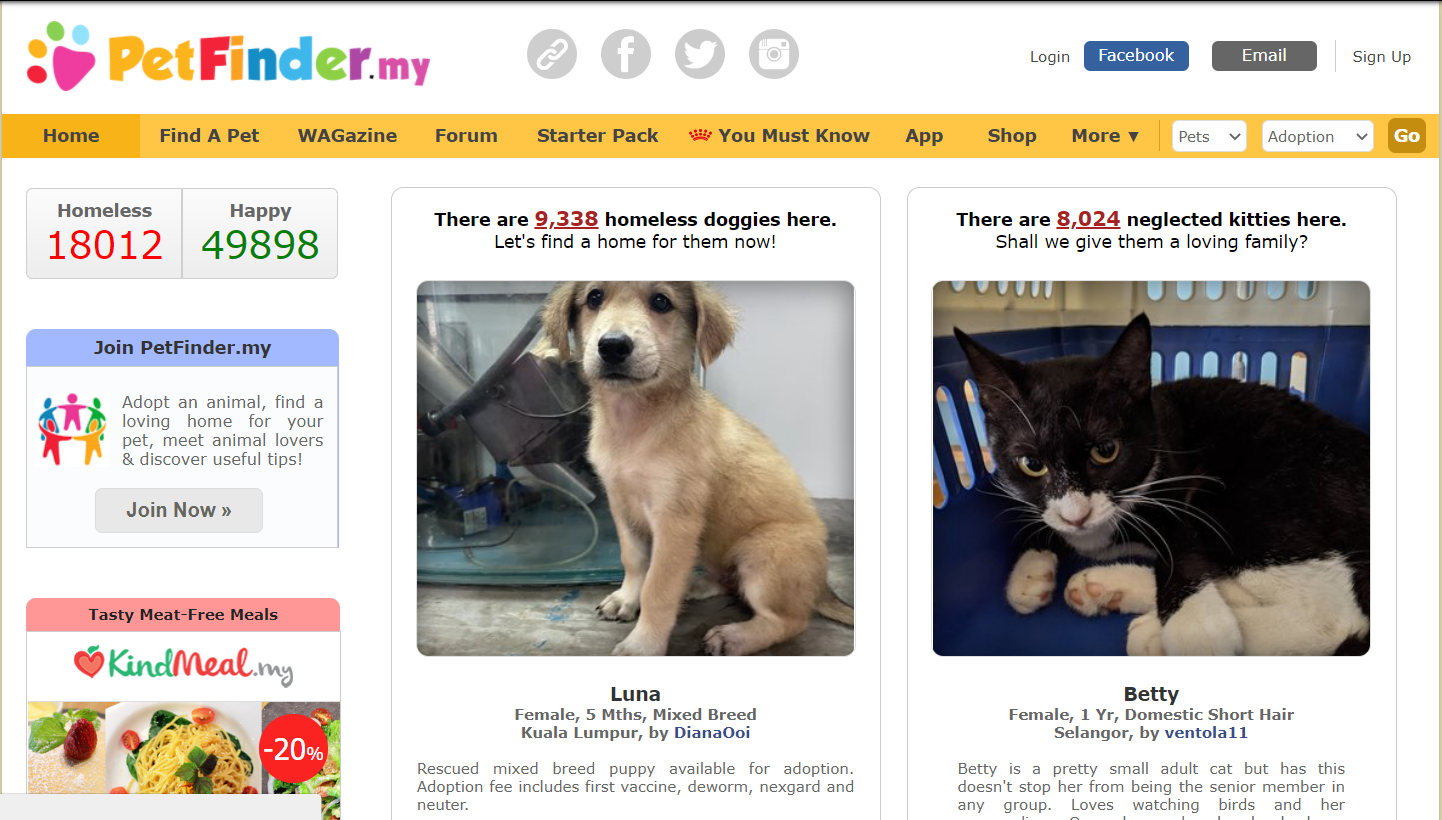
\includegraphics[scale=0.4]{petfinder.png}
	\caption{Скриншот малайзийского сайта}\label{analyse:petfinder}
\end{figure}


\subsection{Описание признаков}

Всего в датасете присутствует 24 признака. Посмотрим на матрицу корреляции (рис. \ref{analyse:corr}). Наибольший коэффициент корреляции имеют переменные Dewormed и Vaccinated --- 0,72. Но этот коэффициент недостаточно высок для того, чтобы утверждать, что данные переменные линейно зависимы. Поэтому нельзя выбрасывать из рассмотрения ни один из этих признаков. Остальные переменные слабо коррелируют между собой.

\begin{figure}[H]
	\centering
	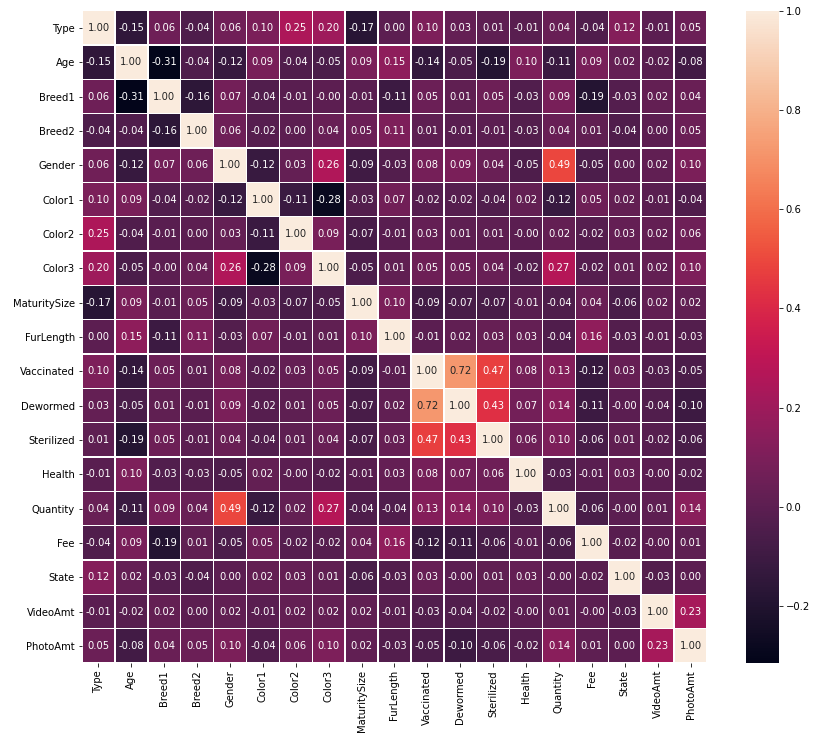
\includegraphics[scale=0.55]{corr.png}
	\caption{Матрица корреляции переменных}\label{analyse:corr}
\end{figure}

Рассмотрим более подробно каждый признак.

PetID --- это уникальный идентификатор питомца. Так как каждый питомец имеет уникальный идентификатор, то не имеет смысла использовать данный признак для обучения модели.

Type --- тип животного. Это категориальная переменная, принимающая два значения: кошка или собака. Количество собак составляет 8132 особи, а кошек — 6861 (рис. \ref{analyse:type}).

\begin{figure}[H]
	\centering
	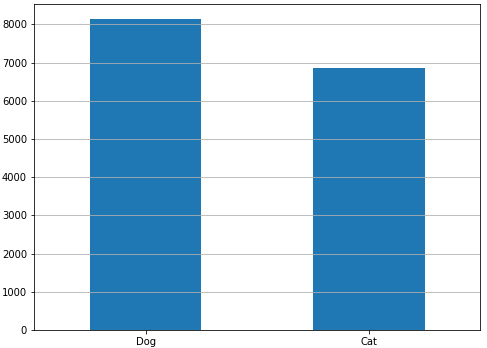
\includegraphics[scale=1.2]{type.png}
	\caption{Распределение кошек и собак в тренировочной выборке}\label{analyse:type}
\end{figure}

Name --- имя питомца. На рисунке \ref{analyse:names} изображены наиболее популярные клички среди кошек и собак. Можно заметить, что большинство людей не придумывали животным имена, а просто называли их “Kitten”, “Puppy” или “No name”. Также была часть животных, имена которых состояли из 1, 2 или 3 символов и не имели смысла. Например, “BB”, “C7C”, “Z4”. 

\begin{figure}[H]
	\centering
	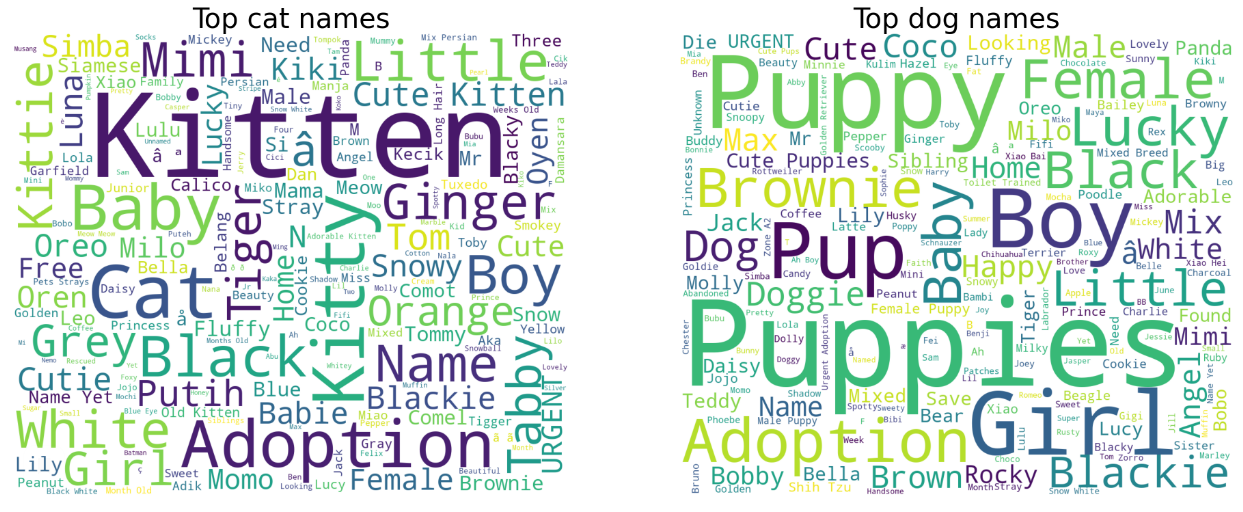
\includegraphics[scale=0.5]{names.png}
	\caption{Наиболее распространённые имена среди кошек и собак}\label{analyse:names}
\end{figure}

Age --- возраст питомца в месяцах.

Breed1 и Breed2 --- переменные, содержащие идентификатор породы, который ссылается на словарь пород breed\_labels.csv. Если питомец чистокровной породы, то в Breed 2 стоит идентификатор 0.

Gender --- категориальная переменная, содержащая пол питомца. Может принимать 3 значения: male, female и mixed. Mixed ставится в том случае, когда в профиле питомцев больше одного. Наибольшее число питомцев имеет мужской пол, наименьшее — смешанный (рис. \ref{analyse:gender})

\begin{figure}[H]
	\centering
	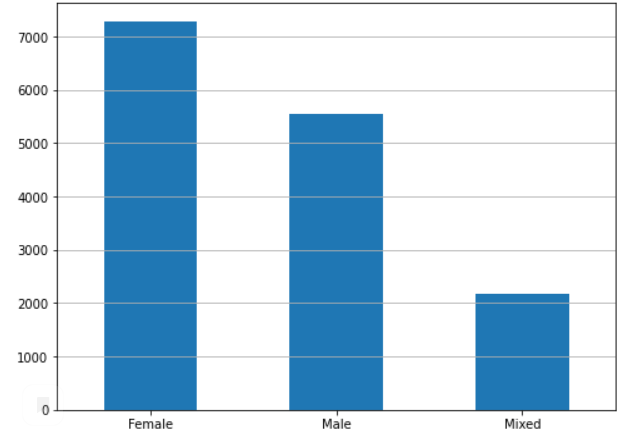
\includegraphics[scale=0.8]{gender.png}
	\caption{Распределение питомцев по полу в train.csv}\label{analyse:gender}
\end{figure}

Переменные Color1, Color2 и Color3 содержат идентификаторы окраса, расшифровка которых находится в файле color\_labels.csv. Если питомец имеет всего один цвет, то в переменных Color2 и Color3 стоит значение 0. Наиболее часто встречаются питомцы коричневого, черно-коричневого и черно-белого цветов (рис. \ref{analyse:color}).

\begin{figure}[H]
	\centering
	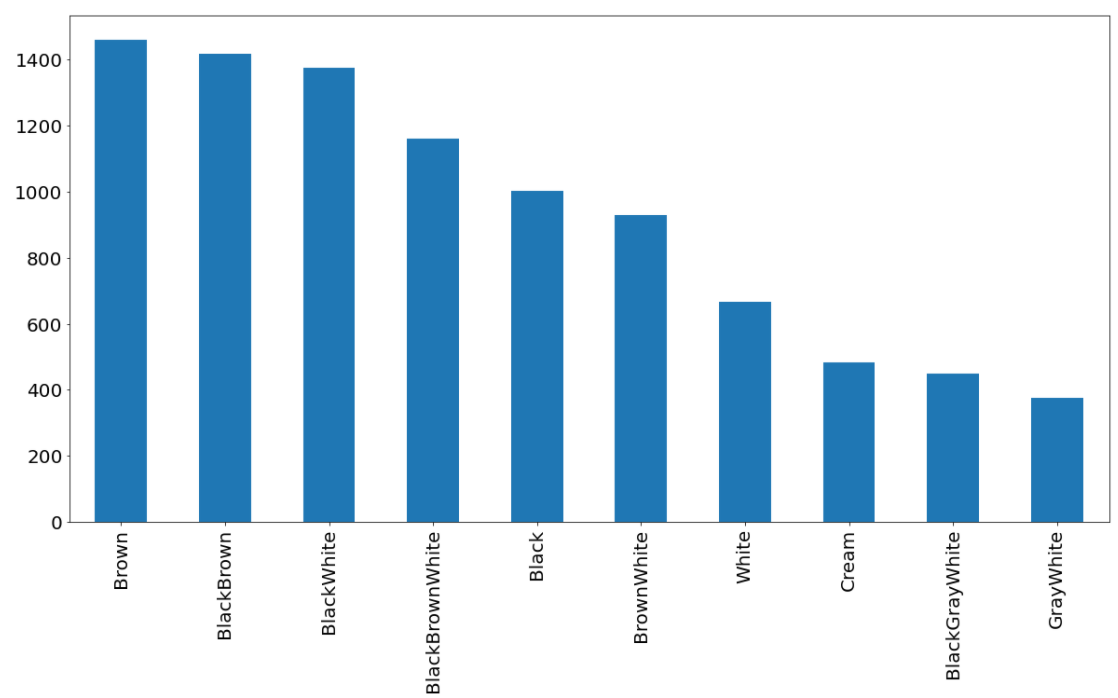
\includegraphics[scale=0.5]{color.png}
	\caption{Наиболее распространнёные комбинации окрасов}\label{analyse:color}
\end{figure}

MaturitySize и FurLength --- категориальные переменные, обозначающие размер в зрелом возрасте и длину шерсти соответственно. MaturitySize принимает 4 значения: ``small'', ``medium'', ``large'' и ``extra large'', а FurLength принимает 3 значения: ``short'', ``medium'', ``long''. Наиболее распространенный размер животного в зрелом возрасте --- средний, а наиболее часто встречающаяся длина шерсти --- короткая (рис. \ref{analyse:sizelength}).

\begin{figure}[H]
	\centering
	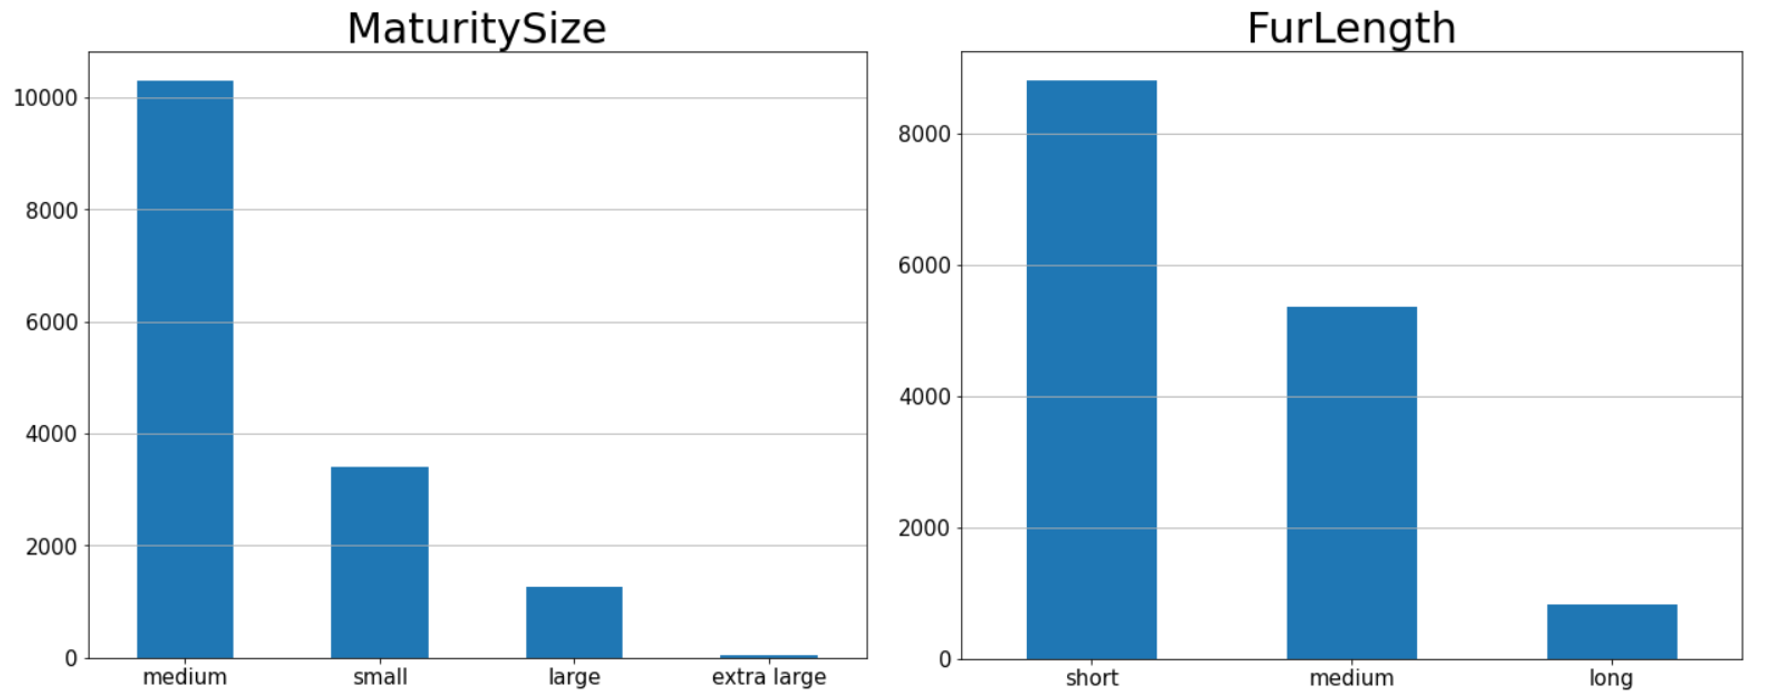
\includegraphics[scale=0.4]{sizelength.png}
	\caption{Наиболее распространнёные комбинации окрасов}\label{analyse:sizelength}
\end{figure}

Также есть 4 категориальных признака, относящихся к здоровью питомца: 

\begin{itemize}
	\item Vaccinated (вакцинировано)
	\item Dewormed (избавлено от гельминтов)
	\item Sterilized (кастрировано)
	\item Health (общее состояние здоровья)
\end{itemize}

Vaccinated, Dewormed и Sterilized принимают 3 значения: ``да'', ``нет'' и ``неизвестно''. Переменная Health также принимает 3 значения: ``Healthy'', ``Minor Injury'', ``Serious Injury''. Большинство животных здоровы, и лишь небольшая часть имеет травмы (рис. \ref{analyse:health}).

\begin{figure}[H]
	\centering
	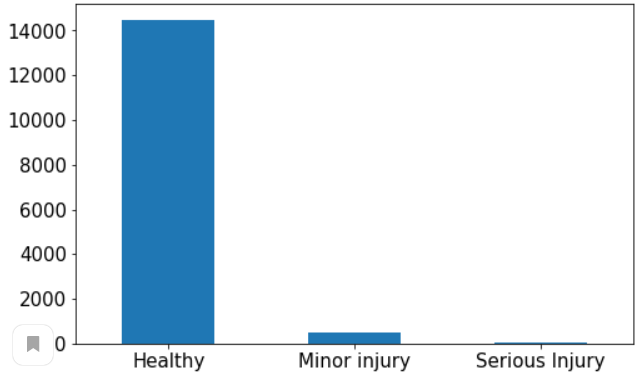
\includegraphics[scale=0.9]{health.png}
	\caption{Состояние здоровья питомцев}\label{analyse:health}
\end{figure}

Quantity --- количество животных в одном профиле. Наибольшее число профилей (11565) содержит одно животное, но также есть записи, где имеется и по 5, и по 10, и даже по 20 животных (рис. \ref{analyse:count}). 

\begin{figure}[H]
	\centering
	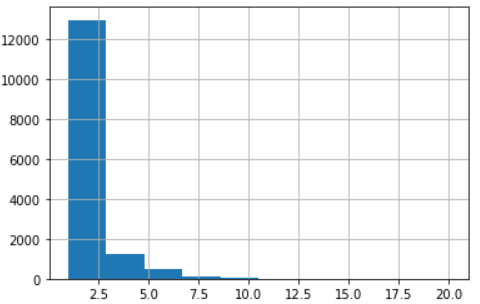
\includegraphics[scale=1]{count.png}
	\caption{Распределение количества животных в одном профиле}\label{analyse:count}
\end{figure}

Fee --- стоимость питомца. В тренировочном датасете 12663 животных отдают бесплатно и 2330 за определенную плату. Причем плата может быть как 10 малайзийских ринггитов, так и 3000 (рис. \ref{analyse:fee}). 

\begin{figure}[H]
	\centering
	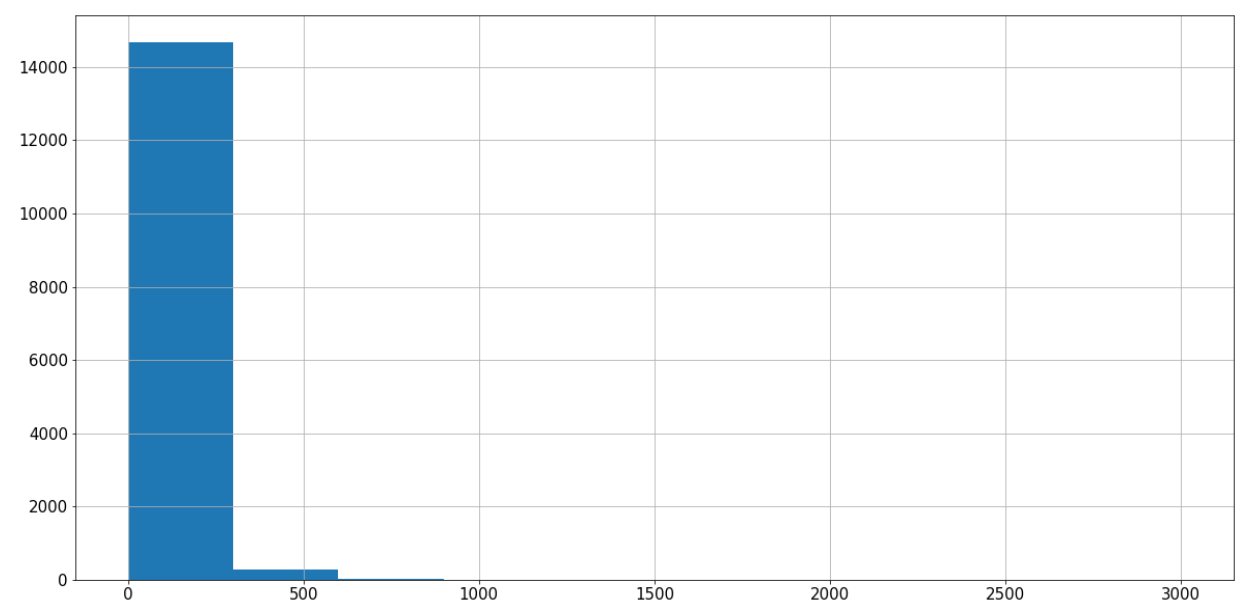
\includegraphics[scale=0.5]{fee.png}
	\caption{Гистограмма стоимости питомца}\label{analyse:fee}
\end{figure}

За плату чаще отдают животных, которые являются чистопородными. Например, за 3000 отдают немецкую овчарку, за 2000 английского бульдога, за 750 персидскую кошку. Но также есть беспородные животные, которых отдают за плату, например, домашнюю длинношерстную кошку за 10 малайзийских ринггитов.

State --- штат в Малайзии, в котором находится питомец. Интересно, что 97\% питомцев находится в 6 штатах, а именно в Selangor, Kuala Lumpur, Pulau Pinang, Johor и Perak (рис. \ref{analyse:state}).

\begin{figure}[H]
	\centering
	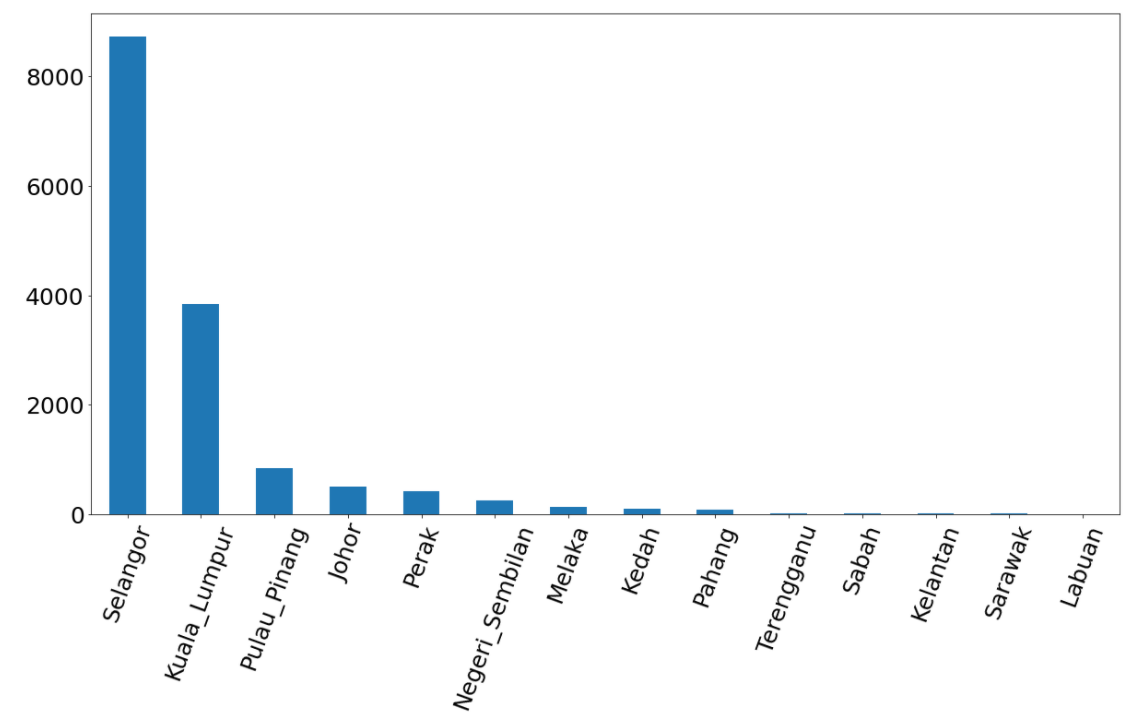
\includegraphics[scale=0.5]{state.png}
	\caption{Количество питомцев в штатах Малайзии}\label{analyse:state}
\end{figure}

RescuerID --- это идентификатор пользователя, который выкладывает профиль животного на сайт. Есть несколько людей или организаций, которые выложили достаточно много объявлений (рис. \ref{analyse:rescuer}). Наибольшее число профилей составило 459.

\begin{figure}[H]
	\centering
	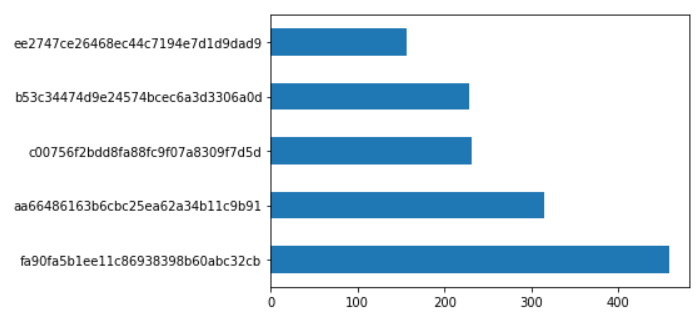
\includegraphics[scale=0.8]{rescuer.png}
	\caption{Количество профилей, которые выложили пользователи}\label{analyse:rescuer}
\end{figure}

VideoAmt и PhotoAmt содержат количество видео и фото, которые содержатся в профиле питомца.
Переменная Description хранит текстовое описание профиля. Основной используемый язык --- английский.

AdoptionSpeed --- это целевая категориальная переменная, которую необходимо предсказать. Всего имеется 5 классов:

\begin{itemize}
	\item 0 --- питомца забрали в первый же день, как профиль был создан
	\item 1 --- питомца забрали в период от 1 до 7 дней после создания профиля
	\item 2 --- питомца забрали в период от 8 до 30 дней после создания профиля
	\item 3 --- питомца забрали в период от 31 до 90 дней после создания профиля
	\item 4 --- питомец не был принят в семью после 90 дней ожидания
\end{itemize}

Для профилей, в которых несколько животных, скорость принятия в семью определяется как скорость, с которой все животные были приняты. 

AdoptionSpeed имеет сильный дисбаланс классов (рис. \ref{analyse:speed}). Количество животных, которых приняли в первый же день (0 класс), составляет 410 особей. А наибольшее число питомцев (4197 особей) находится в 4 классе. Таким образом, количество питомцев в наибольшем классе превышает количество питомцев в наименьшем классе в 10 раз.

\begin{figure}[H]
	\centering
	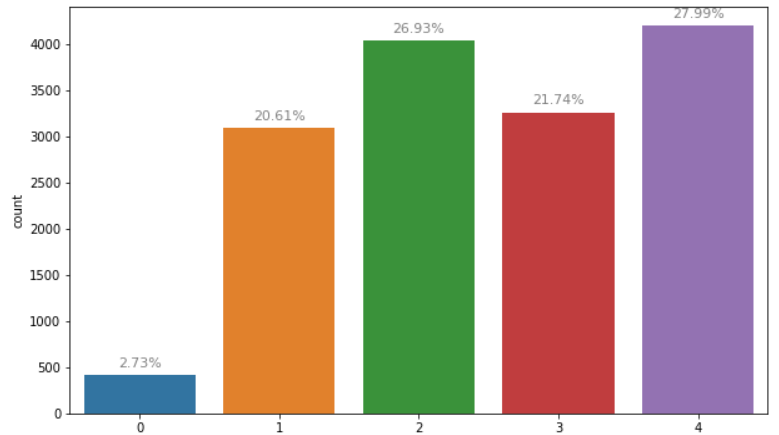
\includegraphics[scale=0.8]{speed.png}
	\caption{Количество питомцев в каждом классе}\label{analyse:speed}
\end{figure}

Для обучения модели все признаки необходимо предобработать, а именно обработать пропущенные значения, найти и обработать выбросы, извлечь признаки из имеющихся данных, закодировать категориальные переменные, привести данные к одной шкале.

\subsection{Обработка пропущенных значений}

В датасете всего 2 переменные содержат пропущенные значения: Name и Description. На рисунке \ref{analyse:empty} пропуски в переменных обозначены белыми чертами. 

\begin{figure}[H]
	\centering
	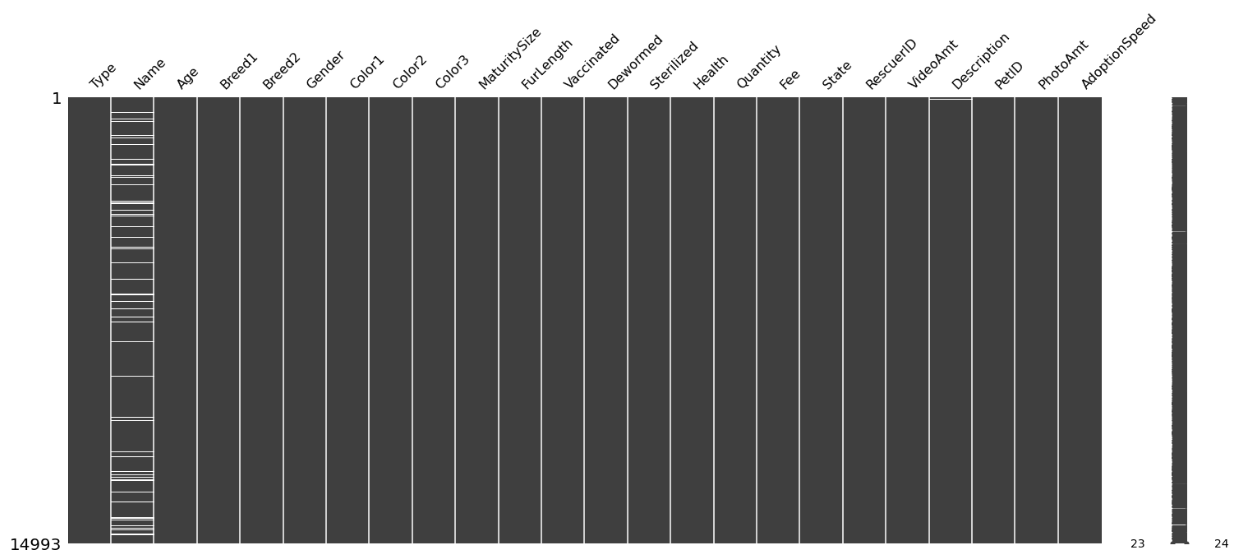
\includegraphics[scale=0.7]{empty.png}
	\caption{Пропущенные значения в данных}\label{analyse:empty}
\end{figure}

Переменная Name содержит 1257 пропусков. Это составляет 8\% от всего датасета. Переменная Description содержит 12 пропущенных значений, что составляет 0.08\% от датасета.
Пропущенные значения необходимо обрабатывать, так как не все модели способны работать с ними. Есть несколько способов борьбы с пропущенными значениями \cite{lib:missingdata}:
\begin{itemize}
	\item Удалить строки, содержащие пропущенные значения
	\item Заменить пропуски выборочным значением
	\item Заменить пропуски средней/медианой/модой
	\item Заполнить случайным значением
\end{itemize}

Удаление пропущенных строк в этом случае не подходит, так как при использовании данного метода значительно сокращается объём датасета и, следовательно, теряется часть информации. Заполнение случайным значением и замена пропусков средней/медианой/модой также не подходят, потому что переменные Name и Description имеют строковый тип. Поэтому остаётся только заменить пропуски выборочным значением. 
Пропуски в Name были заменены значением `No\_name', а в Description пустой строкой. В дальнейшем данные переменные будут дополнительно преобразованы.


\subsection{Детекция и обработка выбросов}

Выбросы — это наблюдения, сильно отличающиеся от остальных наблюдений в выборке. Выбросы необходимо обрабатывать, так как алгоритмы машинного обучения чувствительны к диапазону и распределению переменных \cite{lib:outlier}. Наличие выбросов в данных может привести к увеличению времени обучения, а также к снижению точности.

Для автоматического обнаружения выбросов в данных был использован метод межквартильного расстояния \cite{lib:outlier2}. 

Выбросами в данном случае считаются значения, которые не попадают в диапазон $[Q1 - 1,5 \times (Q3 - Q1), Q3 + 1,5 \times (Q3 - Q1)]$, где $Q1$ и $Q3$ --- первый и третий квартиль соответственно.

Методы обработки выбросов аналогичны методам обработки пропущенных значений. 

В переменной Age достаточно много выбросов (рис. \ref{analyse:ageoutlier}). Максимальное значение возраста составило 255 месяцев. Это больше 21 года, что для кошки и собаки является достаточно большим возрастом. С помощью метода межквартильного расстояния нашли 1501 выброс и заменили их выборочным значением 27, то есть верхней границей полученного диапазона $[-13,\ 27]$. При использовании данного метода необходимо следить за допустимыми значениями переменной. В Age не может быть отрицательных чисел, поэтому значения, которые меньше нуля, необходимо дополнительно обрабатывать, так как они попадают в допустимый диапазон. Но, поскольку в переменной Age не было отрицательных значений, дополнительная обработка не потребовалась.

\begin{figure}[H]
	\centering
	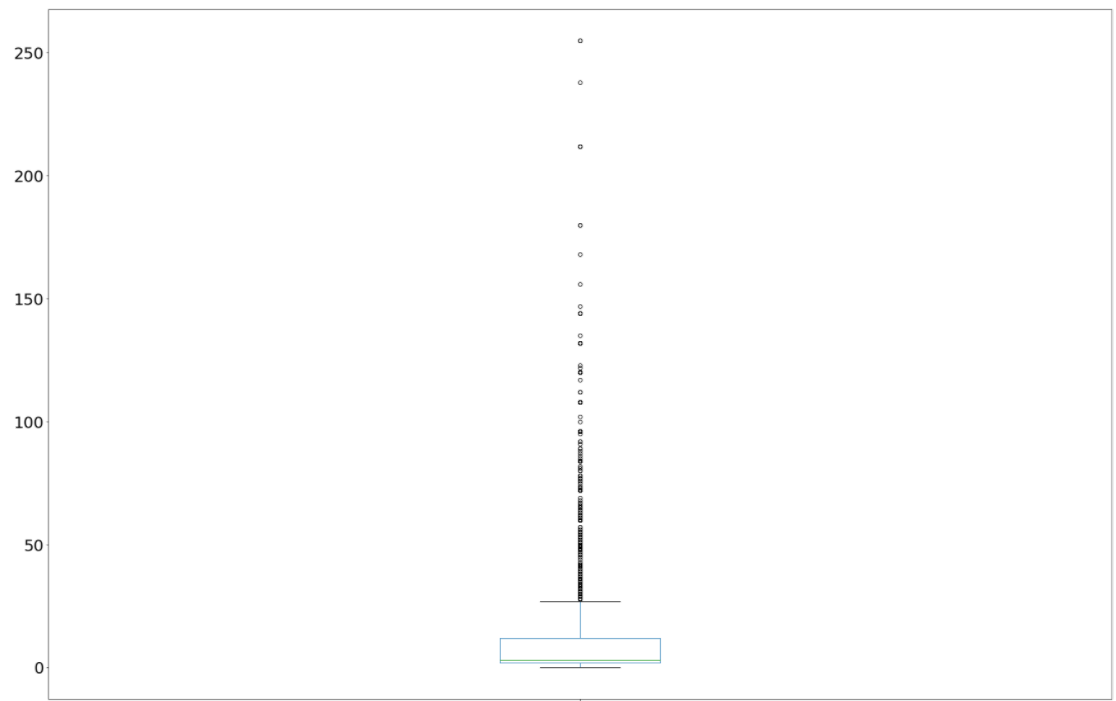
\includegraphics[scale=0.7]{ageoutlier.png}
	\caption{Выбросы в переменной Age}\label{analyse:ageoutlier}
\end{figure}

Аналогично для переменной PhotoAmt было найдено 922 выброса, которые были заменены выборочным значением 9 (рис. \ref{analyse:photooutlier}).

\begin{figure}[H]
	\centering
	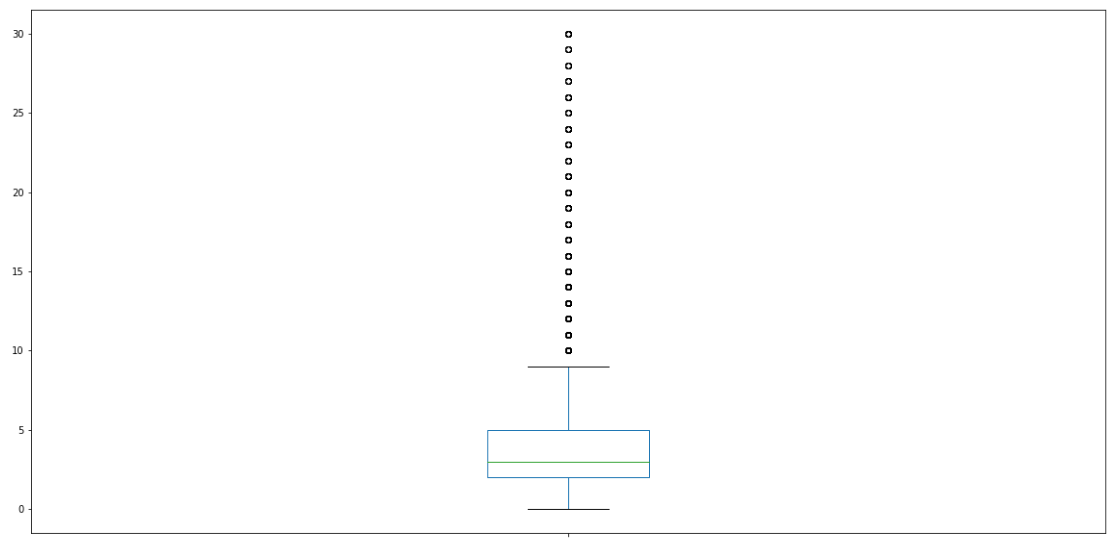
\includegraphics[scale=0.7]{photooutlier.png}
	\caption{Выбросы в переменной PhotoAmt}\label{analyse:photooutlier}
\end{figure}

Также выбросы наблюдаются в переменных Quantity и Fee. Особенностью данных переменных является то, что большая часть значений находится в 1 для Quantity и в 0 для Fee. Из-за этого на графике boxplot (рис. \ref{analyse:feeoutlier}) среднее, медиана, нижняя и верхняя границы, первый и третий квартиль сливаются в одну линию. Если заменить все выбросы верхней границей диапазона (для Quantity --- $[1,\ 1]$, для Fee --- $[0,\ 0]$), то переменная станет константной и не будет иметь значения для обучения модели. Поэтому для обработки данных переменных выбраны две стратегии:
\begin{itemize}
	\item Замена части выбросов выборочным значением
	\item Создание новой переменной, которая оценивает исходную.
\end{itemize}

\begin{figure}[H]
	\centering
	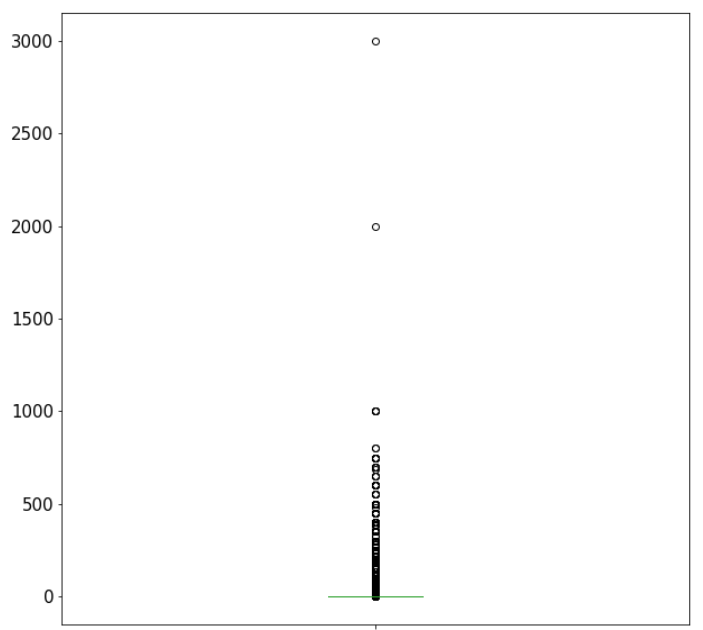
\includegraphics[scale=0.7]{feeoutlier.png}
	\caption{Выбросы в переменной Fee}\label{analyse:feeoutlier}
\end{figure}

При использовании первой стратегии в переменной Quantity заменена часть выбросов, у которых значение больше 5, значением 5, а в переменной Fee заменены значения, превышающие 500, значением 500.

При использовании второй стратегии для Quantity создана новая переменная one\_pet, которая имеет значение 1, если в профиле одно животное, и 0, если животных несколько. Аналогично для переменной Fee создана переменная Free, имеющая значение 1, если животное отдают бесплатно, иначе 0.

Таким образом, обучение будет происходить на двух датасетах, в одном из которых заменены переменные новыми, оценивающими значения, а в другом заменена часть выбросов выборочным значением.


\subsection{Создание новых признаков из имеющихся данных}

Переменная Name имеет строковый формат, и, так как использованные в данной работе модели машинного обучения не умеют работать со строковым типом, то необходимо эту переменную преобразовать. Для этого заменим признак Name новой переменной No\_name, которая будет обозначать, есть ли у животного реальное имя. На этапе обработки пропущенных значений всем значениям равным NaN было поставлено значение `No\_name'. Также в поле Name есть значения, которые обозначают отсутствие имени. Например, ``unnamed'', ``nameless'', ``no name yet''. Ещё есть очень короткие имена, состоящие из 1–3 символов и не имеющие смысла. Все эти значения также были заменены на `No\_name'. Затем новой переменной No\_name присваиваем значение 1, если в Name стоит значение `No\_name', иначе ставим 0. Таким образом, вместо строковой переменной Name получили булеву переменную No\_name (рис. \ref{analyse:hasname}), которую и будем использовать в обучении.

\begin{figure}[H]
	\centering
	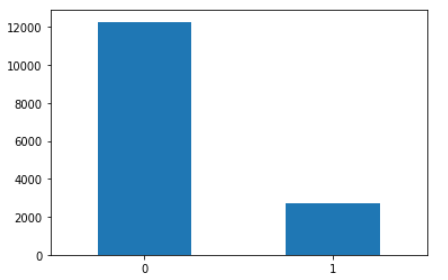
\includegraphics[scale=1]{hasname.png}
	\caption{Число питомцев, имеющих имя и не имеющих имени}\label{analyse:hasname}
\end{figure}

Из переменных Breed1 и Breed2 создана новая переменная Pure\_breed (рис. \ref{analyse:purebreed}), обозначающая, является ли животное породистым или беспородным. Породистому животному присваивается значение 1, беспородному --- 0. Породистым считалось животное, которое в Breed2 имеет значение 0 (то есть нет расшифровки в словаре) и в Breed1 не имеет значения `Mixed\_Breed', `Domestic\_Long\_Hair', `Domestic\_Medium\_Hair' или \\ `Domestic\_Short\_Hair', так как данные виды не считаются породистыми.

\begin{figure}[H]
	\centering
	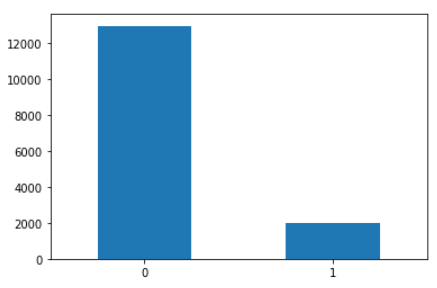
\includegraphics[scale=1]{purebreed.png}
	\caption{Число породистых и беспородных питомцев}\label{analyse:purebreed}
\end{figure}

Переменная RescuerID содержит идентификатор людей или организаций, которые создают профиль питомца на сайте, а также отдают его. Есть идентификаторы, которые создали достаточно много профилей (рис. \ref{analyse:toprescuer}). 

\begin{figure}[H]
	\centering
	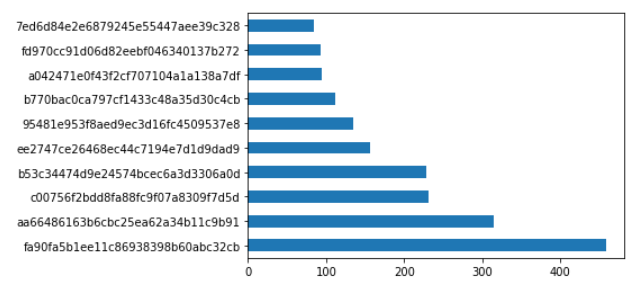
\includegraphics[scale=1]{toprescuer.png}
	\caption{Топ-10 пользователей, создавших наибольшее число профилей}\label{analyse:toprescuer}
\end{figure}

Самое наибольшее --- 459 профилей. Но так как данная переменная строкового типа, а всего уникальных значений 5415, то невозможно считать её категориальной, так как очень сильно расширится пространство признаков при использовании OneHotEncoding, что может негативно сказаться на времени обучения и качестве модели. Поэтому была создана новая переменная RankRescuer. Это переменная обозначает рейтинг пользователей, кто на каком месте по количеству объявлений. То есть пользователь с 459 объявлениями на 1 месте, с 315 --- на 2 и так далее. Если у кого-то совпадает количество объявлений, то они делят одно место. Таким образом, в RankRescuer получилось 61 значение.

Из переменной VideoAmt (количество видео) была создана новая переменная has\_video, которая принимает значение 1, если профиль содержит видео, иначе принимает значение 0. Это было сделано из-за того, что VideoAmt в основном принимает значение 0, а остальные значения считаются выбросами (рис. \ref{analyse:videooutlier}).

\begin{figure}[H]
	\centering
	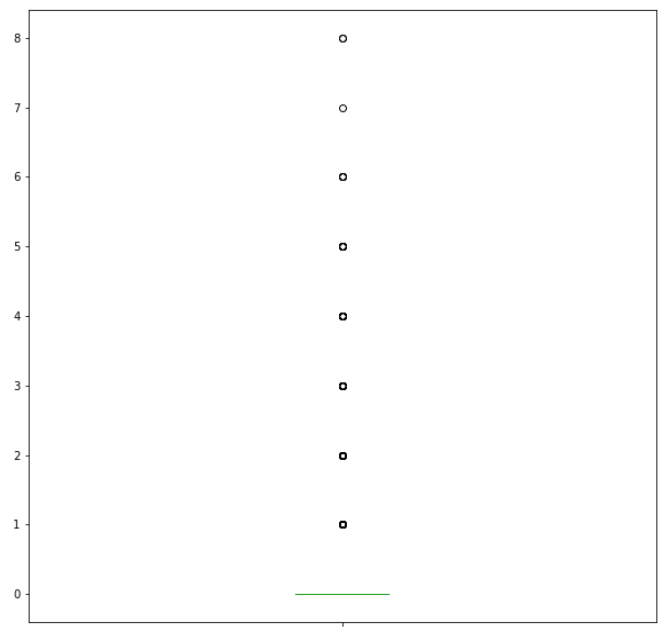
\includegraphics[scale=0.6]{videooutlier.png}
	\caption{Boxplot для VideoAmt}\label{analyse:videooutlier}
\end{figure}

В переменной Description находится описание питомцев. Для каждого описания создатели задачи выполнили анализ эмоциональной окраски текста с помощью Google’s Natural Language API и записали результаты в файлы формата JSON. 

Из информации из этих файлов в данной работе были созданы новые признаки lang, magnitude и score. В переменной lang хранится язык, на котором написаны описания (рис.\ref{analyse:lang}). Модель Google’s Natural Language распознала английский (en), китайский упрощенный (zh), китайский традиционный (zh-Hant) и немецкий (de). Также есть часть наблюдений, где модель не смогла распознать, на каком языке написан текст. Этим наблюдениям присвоено значение `no' в переменной lang. Наблюдений на немецком языке всего 2 штуки, поэтому они были удалены из датасета, чтоб не увеличивать количество категорий. С этой же целью китайский традиционный и китайский упрощенный были объеденены в один язык. 

\begin{figure}[H]
	\centering
	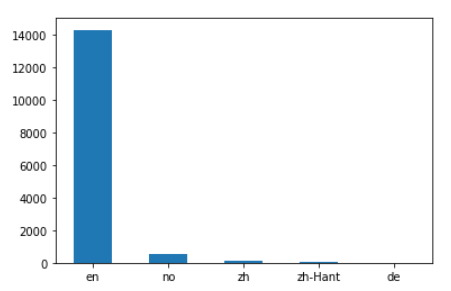
\includegraphics[scale=1.2]{lang.png}
	\caption{Значения переменной lang}\label{analyse:lang}
\end{figure}

Score --- это переменная со значениями из диапазона $[-1,\ 1]$. Отрицательное значение указывает на негативную окраску, положительное --- на положительную. Чем ближе это значение к нулю, тем более текст нейтрален. Magnitude указывает, насколько эмоционален текст \cite{lib:googlelang}.

Примером негативно окрашенного текста является листинг \ref{analyse:neg}. Данный пример имеет score равный -0.7 и magnitude 1.4. Для примера позитивно окрашенного текста (листинг \ref{analyse:pos}) score равняется 0.9, а magnitude 2.7. 

\begin{lstlisting}[language=Python, caption={Пример негативно окрашенного текста}, label=analyse:neg]
The female dog is very pity, she stay at Uncle Kok's house, she 
dislike of other dogs, last 2 week she had borned 11 pupies, but 
now the pupies all died already. Hope someone dog lover can take 
care of the her. Who interested can call to Uncle Kok by this No: 
or to Belinda
\end{lstlisting}

\begin{lstlisting}[language=Python, caption={Пример позитивно окрашенного текста}, label=analyse:pos]
Mocha is very playful and energetic cat. he will play 24/7. He 
is a handsome with amazing fur and white eye color. Eventhough 
he loves playing, he loves to be pampered :) he is toilet trained 
and loves blackwood :)
\end{lstlisting}

Также существуют противоречивые тексты. В этих текстах слов, вносящих позитивный окрас, по количеству примерно столько же, сколько и слов, вносящих негативный окрас. Из-за этого возникает ситуация, когда эмоциональная нагрузка высока, но при этом текст нейтрален. Примером является листинг \ref{analyse:conflict}, где score равен 0, а magnitude — 14.4.

\begin{lstlisting}[language=Python, caption={Пример противоречивого текста}, label=analyse:conflict]
I've lost one of my eye..does anyone love me the way i am? Ding 
Ding is just a 2 months old stray baby who've luckily survived 
from a horrible accident. She is extremely malnourished and 
looked much more smaller size compared to other puppies who have 
the same age. And can you imagine that she is less than 1kg... 
Ding Ding did not lost her life in the accident but unfortunately 
she lost one of her cute and round eyes..She is a very sweet and 
friendly girl, no matter where you go Ding Ding will quietly 
follow you and be by your side all the time, the accident might 
caused her feel extremely insecure. Ding Ding is another innocent 
lives who came to this world..but with the incomplete appearance, 
she has the most beautiful temperament. She would be your perfect 
life companion. Is anyone willing to give a loving home for little 
Ding Ding? She is looking desperately now for a sweet and cozy 
place called HOME. Please don't disappoint her.. Please contact 
(Hwee San)
\end{lstlisting}

Также в данной работе создан признак length\_description, который хранит длину текстового описания питомца. Признаки length\_description и magnitude содержали выбросы, которые были заменены выборочными значениями.
Из файлов, содержащих метаданные, которые создатели задачи получили, обработав изображения с помощью Google Vision API, в данной работе были получены две переменные object\_in\_img и score\_in\_img. Переменная object\_in\_img содержит информацию о том, нашла ли модель кошку или собаку на изображении, или же определила что-то другое. В случае кошки или собаки переменная имеет значения `cat' или `dog', иначе значение `no' (рис. \ref{analyse:objectimg}). Переменная score\_in\_img обозначает уверенность модели в своём предсказании (рис. \ref{analyse:scoreimg}). В большинстве случаев модель Google Vision предсказала объект на изображении с точностью более 95\%.

\begin{figure}[H]
	\centering
	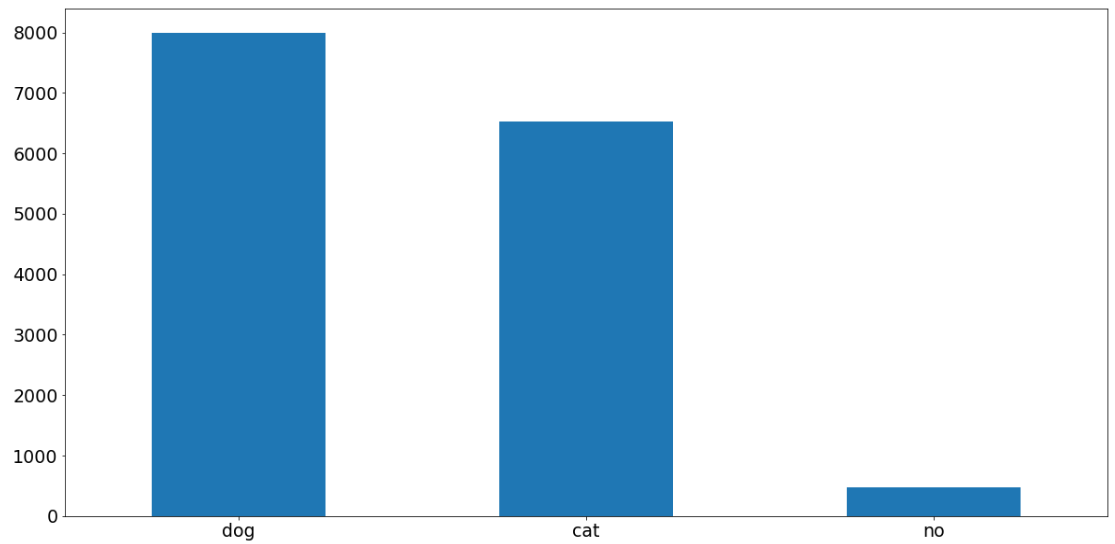
\includegraphics[scale=0.5]{objectimg.png}
	\caption{Значения переменной object\_in\_img}\label{analyse:objectimg}
\end{figure}

\begin{figure}[H]
	\centering
	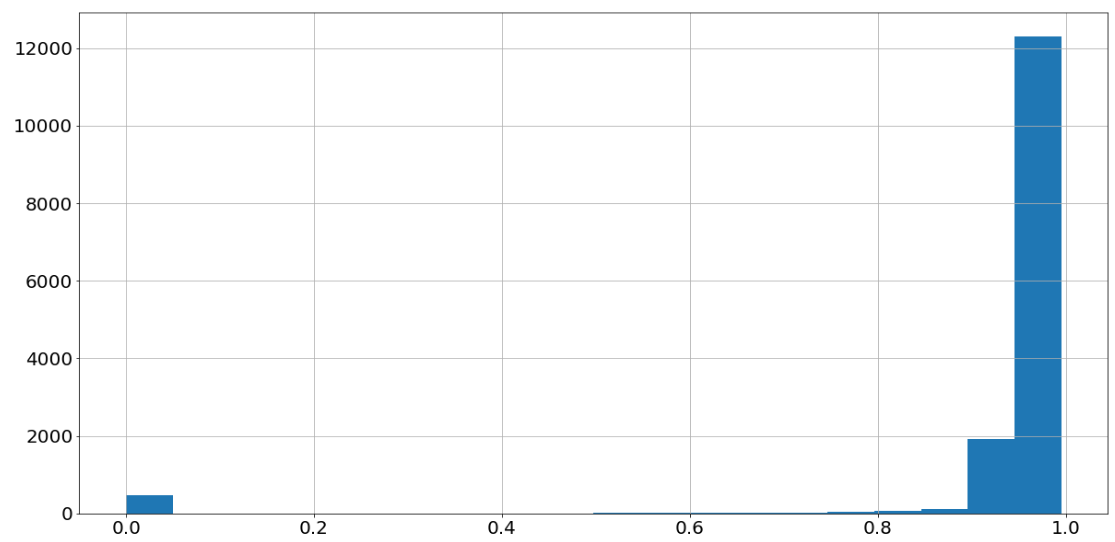
\includegraphics[scale=0.5]{scoreimg.png}
	\caption{Гистограмма частот переменной score\_in\_img}\label{analyse:scoreimg}
\end{figure}



\subsection{Кодирование категориальных переменных}

Многие алгоритмы машинного обучения не способны напрямую работать с категориальными переменными, поэтому их необходимо обработать специальным образом, то есть закодировать. Также кодирование категориальных переменных может значительно улучшить качество моделей. Существует множество различных способов кодировки переменных, но в данной работе используется три наиболее распространенных способа \cite{lib:encode}:
\begin{itemize}
	\item Прямое кодирование
	\item One Hot Encoding
	\item Target Encoding
\end{itemize}

Для проведения прямого кодирования использовался LabelEncoder() из библиотеки sklearn. Данный способ каждой категории ставит в соответствие целое число. Этот метод хорош тем, что он интуитивно понятен и не расширяет пространство признаков. Минусом является то, что если категориальные переменные не являются порядковыми, то модель, обучаясь на таких данных, может найти взаимосвязь там, где её нет, и из-за этого качество модели может быть хуже, чем при других методах кодирования.

Для реализации метода One Hot Encoding использовалась функция get\_dummies из библиотеки pandas. Данный метод для каждого значения категориальной переменной создаёт отдельный столбец, в который записывает 0 или 1 в зависимости от того, присутствует ли такое значение в данном наблюдении. Данный метод хорошо интерпретируется, но при этом очень сильно расширяет пространство признаков. 

Target Encoding был применен с использованием TargetEncoder() из библиотеки category\_encoders. Отличительной особенностью данного метода является то, что для кодирования категориальных переменных используется целевая переменная (см. формула 1). Он прост и быстр, а также не увеличивает пространство признаков. Но минусом является то, что метод сильно зависит от распределения целевой переменной и склонен к переобучению. Также этот метод сильно зависит от данных и показывает значительные улучшения только в некоторых случаях \cite{lib:encoding}.

Target Encoding категориальной переменной производится по формуле \ref{eq:tar} \cite{lib:tarencode}:

\begin{equation}\label{eq:tar}
	x^i_k=prior \times (1-s)+s \times \frac{n^i_k}{n_k},
\end{equation}

\begin{equation*}
	\text{где } s = \frac{1}{1 + \exp \left( \frac{-n_k-mdl}{\alpha} \right)}
\end{equation*}
где $prior$ --- среднее значение целевой переменной;  $n_k$ --- общее число строк, отнесенных к категории $k$; $n^i_k$ --- число строк, отнесённых к категории $k$ и принимающих $i$ значение целевой переменной; $mdl$ --- минимум в категориальной переменной; $\alpha$ --- коэффициент регуляризации.


\subsection{Шкалирование переменных}

Многие алгоритмы машинного обучения показывают лучшие результаты и скорость работы, если признаки находятся в относительно сходном масштабе или близки к нормальному распределению \cite{lib:standardize}.  Примерами таких алгоритмов могут служить логистическая регрессия, k ближайших соседей, нейронные сети, SVM (support vector machine) и другие. Также чувствительны к шкалированию алгоритмы, основанные на методе градиентного спуска.

В данной работе использовался StandardScaler() из библиотеки sklearn. Данный вид шкалирования стремится привести данные к нормальному распределению, то есть распределению, у которого математическое ожидание находится в районе нуля, а среднеквадратичное отклонение в районе единицы. Преобразование происходит по формуле \ref{eq:1} \cite{lib:sklearnstandard}:

\begin{equation}\label{eq:1}
	z = \frac{x-u}{s},
\end{equation}
где $u$ --- математическое ожидание, $s$ --- среднеквадратичное отклонение, $x$ --- значение наблюдения стандартизируемого признака.

Данный метод чувствителен к выбросам, но так как все выбросы были обработаны, то метод применим.

\begin{figure}[H]
	\centering
	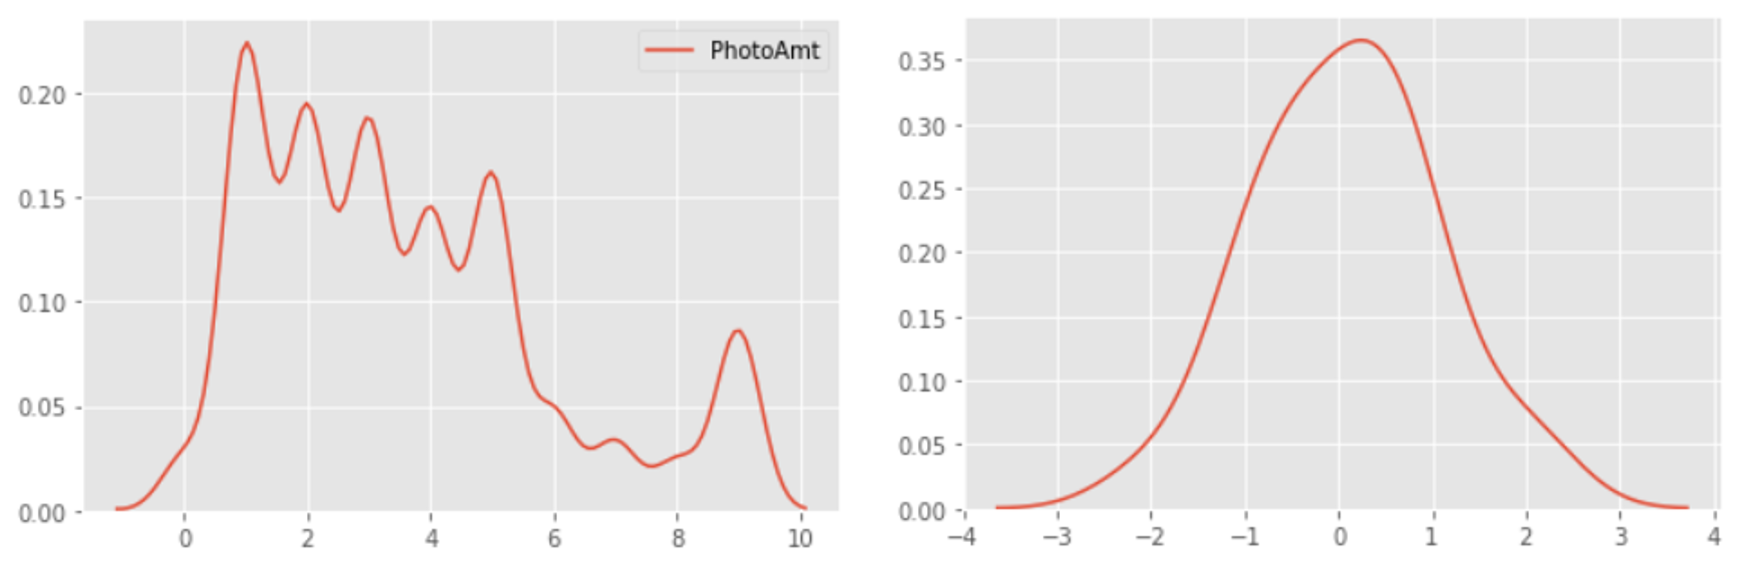
\includegraphics[scale=0.4]{photoamt.png}
	\caption{Распределение переменной PhotoAmt до и после шкалирования}\label{analyse:photoamt}
\end{figure}

На рисунке \ref{analyse:photoamt} слева изображено распределение переменной PhotoAmt до применения StandardScaler(), справа --- после. Можно наблюдать, что распределение переменной после шкалирования действительно близко к нормальному.

%=======================
\newpage
\section{Используемая метрика}

Для проверки качества модели на тестовой выборке и подбора гиперпараметров на кросс-валидации создателями задачи предложена к использованию метрика взвешенная квадратичная каппа (Quadratic Weighted Kappa). Поэтому именно её будем использовать в данной работе. 

Взвешенная квадратичная каппа --- это показатель, который применяется для расчета степени сходства между предсказанными и фактическими значениями \cite{lib:kappa1}. Данная метрика показывает, насколько лучше построенный классификатор работает по сравнению с классификатором, который просто случайным образом угадывает в соответствии с распределением переменной.

Взвешенная квадратичная каппа применяется в тех случаях, когда значения переменной упорядочены. То есть 0 класс меньше 1 класса, 1 меньше 2 и так далее. В данной задаче это именно так, потому что значения целевой переменной AdoptionSpeed обозначают временные промежутки. 

Значение квадратичной взвешенной каппы находится в диапазоне от $-1$ до $1$ \cite{lib:kappa2}. Значение 1 может получиться только тогда, когда предсказанные и истинные значения полностью совпадают. Значение каппы 0 обозначает, что классы были предсказаны случайно в соответствии с распределением целевой переменной. Значение $-1$ может получиться, если предсказанные значения наиболее далеки от истинных. Например, если все фактические значения равны 0, а предсказанные --- 4.

Для проведения оценки моделей с помощью метрики Quadratic Weighted Kappa в работе была использована cohen\_kappa\_score, которая уже реализована в библиотеке sklearn. Для того, чтобы установить веса как квадратичные взвешенные, в функции был установлен параметр weights='quadratic'.


%=======================
\newpage
\section{Использованные модели}

Для предсказания класса скорости принятия животного в семью необходимо построить модели, классифицирующие наблюдения. В зависимости от предобработки данных получилось 6 датасетов. Для краткости введём обозначения: 

\begin{itemize}
	\item B --- датасет, где были заменены выбросы в Fee и Quantity на булевы переменные
	\item B\_ohe --- датасет, где были заменены выбросы в Fee и Quantity на булевы переменные и применены One Hot Encoding и StandardScaler
	\item B\_tar --- датасет, где были заменены выбросы в Fee и Quantity на булевы переменные и применены TargetEncoder и StandardScaler
	\item N — датасет, где была заменена часть выбросов в Fee и Quantity на выборочное значение 
	\item N\_ohe --- датасет, где была заменена часть выбросов в Fee и Quantity на выборочное значение и применены One Hot Encoding и StandardScaler
	\item N\_tar --- датасет, где была заменена часть выбросов в Fee и Quantity на выборочное значение и применены TargetEncoder и StandardScaler
\end{itemize}

Все эти датасеты были предварительно разделены на тренировочную и тестовую выборки в соотношении 4:1 с помощью функции train\_test\_split из библиотеки sklearn. Так как целевая переменная имеет сильный дисбаланс, то при разделении на тренировочную и тестовую выборки была выполнена стратификация по целевой переменной для того, чтобы сохранить распределение классов.

Обучим различные алгоритмы машинного обучения на этих данных и сравним их эффективность. Также выполним подбор оптимальных параметров с помощью GridSearchCV или RandomizedSearchCV из библиотеки sklearn. В качестве генератора перекрестной проверки будем использовать StratifiedKFold.


\subsection{Baseline}

Первым делом было построено наивное предсказание (листинг \ref{models:baselinecode}), которое случайным образом предсказывает класс с учетом распределения целевой переменной (рис. \ref{models:baseline}).

\begin{lstlisting}[language=Python, caption={Python, создание baseline}, label=models:baselinecode]
y_naive_pred = np.random.choice(
	[4., 2., 3., 1., 0.], 
	len(y_test), 
	p=y_train.value_counts(normalize=True).values)
\end{lstlisting}

\begin{figure}[H]
	\centering
	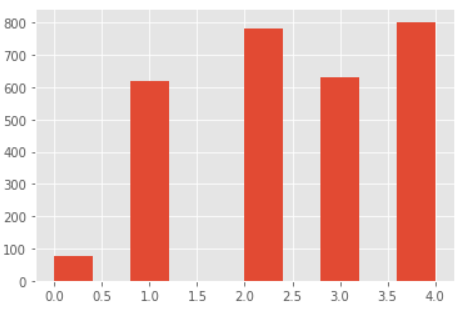
\includegraphics[scale=1]{baseline.png}
	\caption{Распределение предсказанных значений baseline}\label{models:baseline}
\end{figure}

Данная модель показала качество 0.03, что близко к нулю и подтверждает то, что взвешенная квадратичная каппа в случае случайного предсказания равна 0.

Baseline является отправной точкой для построения других моделей машинного обучения. Если качество модели хуже, чем у baseline, то данная модель предсказывает хуже, чем случайное угадывание в соответствии с распределением.


\subsection{Дерево решений}

Дерево решений --- это модель, имеющая структуру дерева и позволяющая решать задачи классификации и регрессии. Данная модель используется в тех случаях, когда нужна простая и четкая интерпретация, так как дерево решений основано на решающих правилах вида <<если..., то...>>. 
 
Преимуществами данного метода являются хорошая интерпретируемость, быстрый процесс обучения, поддержка категориальных признаков, возможность визуализации.

Но в чистом виде деревья редко применяются на практике, так как они склонны к переобучению, чувствительны к выбросам. Также нет гарантии, что найденное дерево является оптимальным решением \cite{lib:trees}. Гораздо чаще деревья используются в ансамблях.

В качестве модели использовалась функция DecisionTreeClassifier из библиотеки sklearn.

На рисунке \ref{models:tree} изображено дерево, построенное на датасете B, с глубиной 1. В качестве решающего правила модель использовала утверждение <<Если RankRescuer <= 47.5, то...>>. Данная модель показала качество на тестовой выборке $-0.03$, что даже хуже, чем если бы модель предсказывала случайным образом в соответствии с распределением целевой переменной.

\begin{figure}[H]
	\centering
	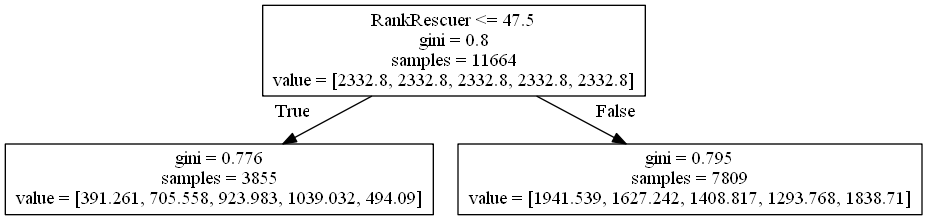
\includegraphics[scale=0.7]{tree.png}
	\caption{Дерево решений с глубиной 1}\label{models:tree}
\end{figure}

Если обучить модели без настройки параметров, то наилучшее качество показала модель, построенная на основе признаков из датасета, в котором выбросы в переменных Fee и Quantity были заменены выборочным значением, а также не применялись методы кодирования категориальных переменных и методы шкалирования (таблица \ref{models:table1}).

\begin{table}[H]
	\centering
	\caption{Качество дерева решений на тестовой выборке до подбора параметров}\label{models:table1}
	\begin{tabular}{cccc}
		\hline
		датасет & качество	& датасет & качество \\
		\hline
		B &	0.19 &	N &	0.25\\
		B\_ohe &	0.19 &	N\_ohe &	0.22\\
		B\_tar &	0.24 &	N\_tar &	0.24\\
		\hline
	\end{tabular}
\end{table}

Попробуем улучшить качество моделей с помощью подбора гиперпараметров по сетке с использованием GridSearchCV. Зададим максимальную глубину от 2 до 30, минимальное количество наблюдений в листах дерева от 2 до 11, веса классов (class\_weight) сбалансированные и несбалансированные, а в качестве критерия принятия решений gini и entropy.

\begin{table}[H]
	\centering
	\caption{Качество дерева решений на тестовой выборке после подбора параметров}\label{models:table2}
	\begin{tabular}{cccc}
		\hline
		датасет & качество	& датасет & качество \\
		\hline
		B &	0.29 &	N &	0.33 \\
		B\_ohe & 0.29 &	N\_ohe & 0.34\\
		B\_tar & 0.28 & N\_tar & 0.32 \\
		\hline
	\end{tabular}
\end{table}

После настройки гиперпараметров качество моделей значительно улучшилось (таблица \ref{models:table2}). При этом качество не сильно отличается в зависимости от кодирования и шкалирования, из чего можно сделать вывод, что деревья решений не сильно зависят от данных методов предобработки. Модели, построенные на датасетах, в которых выбросы были заменены выборочным значением, показали лучшие результаты, чем те, что были построены на датасетах, в которых выбросы заменены на булевы переменные. 


\subsection{Логистическая регрессия}

Логистическая регрессия --- это линейная модель, которая позволяет оценивать вероятности принадлежности объектов классам \cite{lib:logreg}.

Данный метод прост в реализации, не требует больших вычислительных мощностей, есть возможность узнать вероятность принадлежности объекта к какому-либо классу. Также данный метод эффективен, когда классы линейно разделимы. Недостатками является то, что логистическая регрессия неспособна решать нелинейные задачи, чувствительна к выбросам, а также склонна к переобучению \cite{lib:logreg2}.

В качестве модели использовалась функция LogisticRegression() из библиотеки sklearn.

При обучении без настройки параметров (таблица \ref{models:table3}), модели, обученные на датасетах без кодирования категориальных переменных и без шкалирования, показали значительно худшие результаты, чем модели, которые были обучены на датасетах с дополнительной предобработкой.

\begin{table}[H]
	\centering
	\caption{Качество логистической регрессии на тестовой выборке до подбора параметров}\label{models:table3}
	\begin{tabular}{cccc}
		\hline
		датасет & качество	& датасет & качество \\
		\hline
		B &	0.12 &	N &	0.17 \\
		B\_ohe & 0.29 &	N\_ohe & 0.31\\
		B\_tar & 0.29 & N\_tar & 0.32 \\
		\hline
	\end{tabular}
\end{table}

Подбор параметров будет проводится по сетке GridSearchCV со следующими параметрами: коэффициент регуляризации C со значениями 0.1, 0.3, 0.5 и 1.0, веса (class\_weight) сбалансированные и несбалансированные и алгоритм оптимизации `newton-cg', `lbfgs', `liblinear' и `sag'. После подбора наилучших параметров были получены результаты работы модели, приведенные в таблице \ref{models:table4}.

\begin{table}[H]
	\centering
\caption{Качество логистической регрессии на тестовой выборке после подбора параметров}\label{models:table4}
\begin{tabular}{cccc}
	\hline
	датасет & качество	& датасет & качество \\
	\hline
	B &	0.26 &	N &	0.28 \\
	B\_ohe & 0.29 &	N\_ohe & 0.31\\
	B\_tar & 0.29 & N\_tar & 0.32 \\
	\hline
\end{tabular}
\end{table}

После подбора параметров качество моделей получилось чуть хуже, чем у решающих деревьев.


\subsection{Случайный лес}

Случайный лес --- это модель, которая состоит из нескольких решающих деревьев. Все деревья в данной модели строятся независимо друг от друга (данная стратегия ансамблирования моделей называется бэггингом), а решение о том, к какому классу отнести, принимается голосованием по большинству. Каждое дерево в алгоритме обучается на случайной подвыборке, а при разделении узлов выбираются случайные наборы параметров. Эти особенности данного алгоритма позволяют достигать лучших результатов, чем при использовании одного решающего дерева \cite{lib:randomforest}.

Преимуществами данного алгоритма является то, что он практически нечувствителен к выбросам за счет обучения на случайных подвыборках, не чувствителен к масштабу данных, не требует тщательной настройки параметров, способен эффективно обрабатывать данные, содержащие большое число признаков и классов, а также редко переобучается. Ещё одним преимуществом является возможность распараллеливания вычислений, так как базовые модели учатся независимо друг от друга. Недостатками же является то, что сложно интерпретировать результаты работы модели, случайный лес работает хуже линейных моделей в случае большого числа разреженных признаков (например, создание «мешка слов» в обработке текстов), склонен к переобучению на зашумленных данных, а также требует большого объёма памяти для хранения, а именно O(K), где K ---  число решающих деревьев \cite{lib:randomforest2}.

В качестве модели использовалась функция RandomForestClassifier() из библиотеки sklearn. Без настройки параметров данная модель показала значительно лучшее качество по сравнению с логистической регрессией и деревом решений (Таблица \ref{models:table5}). Также нет особой разницы в качестве между методами кодирования категориальных переменных. Все показали примерно одинаковое качество. Но модели, в датасетах которых выбросы были заменены выборочным значением, показали лучшие результаты, чем при замене булевыми переменными.

\begin{table}[H]
	\centering
	\caption{Качество случайного леса на тестовой выборке до подбора параметров}\label{models:table5}
	\begin{tabular}{cccc}
		\hline
		датасет & качество	& датасет & качество \\
		\hline
		B &	0.38 &	N &	0.42 \\
		B\_ohe & 0.37 &	N\_ohe & 0.41\\
		B\_tar & 0.39 & N\_tar & 0.42 \\
		\hline
	\end{tabular}
\end{table}

Подбор параметров производился по сетке со следующими параметрами: количество решающих деревьев 100, 200 и 300, максимальная глубина каждого дерева от 2 до 20, минимальное количество наблюдений в листьях 3, 5, 7, 9, 11, веса сбалансированные и несбалансированные, а также критерий по которому выполняется разбиение gini и entropy.

\begin{table}[H]
	\centering
	\caption{Качество случайного леса на тестовой выборке после подбора параметров}\label{models:table6}
	\begin{tabular}{cccc}
		\hline
		датасет & качество	& датасет & качество \\
		\hline
		B &	0.38 &	N &	0.41 \\
		B\_ohe & 0.38 &	N\_ohe & 0.42\\
		B\_tar & 0.40 & N\_tar & 0.42 \\
		\hline
	\end{tabular}
\end{table}

После настройки параметров качество моделей изменилось на 0.01, что не является значительным повышением качества (таблица \ref{models:table6}). Это подтверждает тот факт, что данная модель не требует тщательной настройки параметров.

\subsection{Градиентный бустинг}

Градиентный бустинг --- это стратегия построения ансамблей моделей, в которой базовые предсказатели построены не независимо как в бэггинге, а последовательно. Главная идея заключается в том, что каждая последующая базовая модель учится на ошибках предыдущей. А оптимизация функции потерь происходит методом градиентного спуска \cite{lib:gradboost}.

Преимуществами данного метода является поддержка различных функций потерь и множества различных гиперпараметров, градиентный бустинг работает хорошо как с непрерывными, так и с категориальными переменными, может обрабатывать пропущенные значения. Недостатками является склонность к переобучению, большие временные и вычислительные затраты из-за большого числа базовых предсказателей, сложность настройки гиперпараметров \cite{lib:gradboost2}.

В качестве моделей, реализующих алгоритм градиентного бустинга, использовались следующие классификаторы: GradientBoostingClassifier() из библиотеки sklearn, XGBClassifier() из библиотеки XGBoost, а также LGBMClassifier() из библиотеки LightGBM.

\begin{table}[H]
	\centering
	\caption{Качество градиентного бустинга на тестовой выборке}\label{models:table7}
	\begin{tabular}{cccc}
		\hline
		датасет & модель & \multicolumn{2}{c}{качество} \\
		& & до настройки & после настройки \\
		\hline
		B & GradientBoostingClassifier() & 0.37 & 0.36 \\
		& XGBClassifier() & 0.36 & 0.37 \\
		& LGBMClassifier() & 0.37 & 0.38 \\
		\hline
		B\_ohe & GradientBoostingClassifier() & 0.37 & 0.38 \\
		& XGBClassifier() & 0.37 & 0.37 \\
		& LGBMClassifier() & 0.36 & 0.37 \\
		\hline
		B\_tar & GradientBoostingClassifier() & 0.36 & 0.37 \\
		& XGBClassifier() & 0.38 & 0.38 \\
		& LGBMClassifier() & 0.39 & 0.38 \\
		\hline
		N & GradientBoostingClassifier() & 0.38 & 0.39 \\
		& XGBClassifier() & 0.42 & 0.42 \\
		& LGBMClassifier() & 0.43 & 0.42 \\
		\hline
		N\_ohe & GradientBoostingClassifier() & 0.39 & 0.41 \\
		& XGBClassifier() & 0.42 & 0.42 \\
		& LGBMClassifier() & 0.42 & 0.42 \\
		\hline
		N\_tar & GradientBoostingClassifier() & 0.40 & 0.41 \\
		& XGBClassifier() & 0.42 & 0.42 \\
		& LGBMClassifier() & 0.43 & 0.42 \\ 
		\hline
	\end{tabular}
\end{table}

Настройка гиперпараметров проходила по сетке, содержащей следующие параметры: максимальная глубина дерева 1, 3, 5, 7 и 9, количество базовых предсказателей 50, 100, 200, 300 и коэффициент скорости обучения 1.0, 0.5, 0.1, 0.05, 0.025, 0.01 и 0.005.

Все три модели после настройки гиперпараметров не дали значительных улучшений в качестве (таблица \ref{models:table7}). Между методами кодирования категориальных переменных также как и в модели случайного леса не наблюдается значительных различий в качестве. И также как и во всех предыдущих рассматриваемых моделях качество лучше на датасетах, в которых выбросы в переменных Fee и Quantity были заменены на выборочные значения, а не на новые булевы переменные.

%=======================
\newpage
\section{Классификация только с использованием текстовых признаков}

\subsection{Предобработка текстов и выделение признаков}

Для того, чтобы предсказать, к какому классу «скорости принятия» относится тот или иной питомец, основываясь только на текстовых признаках, был создан новый датасет, состоящий только из колонок Description и AdoptionSpeed исходного датасета train.csv.

Предобработка текста происходила в несколько этапов:

\begin{itemize}
	\item Токенизация
	\item Нормализация
	\item Удаление стоп-слов
	\item Стемминг и Лемматизация
	\item Векторизация
\end{itemize}

Токенизация --- это разделение длинного текста на более мелкие части, которые называются токенами. Это могут быть абзацы, отдельные предложения или же слова. В данной работе использовался такой метод токенизации, как деление на слова.
 
Далее каждое описание было нормализовано, то есть все слова приведены к нижнему регистру, а также удалены знаки препинания. 

Наличие стоп-слов в тексте, а именно местоимений, союзов, артиклей, может добавить много шума при обучении моделей. Эти слова очень часто встречаются в текстах и не несут никакой смысловой нагрузки, поэтому их необходимо удалить. Для удаления использовался уже готовый список английских стоп-слов из библиотеки nltk, куда входит 179 уникальных значений. К примеру, `i', `me', `our', `myself', `the', `because' и другие. 

Также тексты могут содержать различные грамматические формы одного слова или однокоренные слова. Поэтому их необходимо привести к нормальной форме. Для этих целей используются такие методы как стемминг и лемматизация \cite{lib:stemlem}. Главное отличие лемматизации от стемминга заключается в том, что стемминг просто обрезает у слов приставки и окончания по заданным правилам, даже если этих обрезанных слов не существует, а лемматизация использует морфологический анализ и контекст для приведения слов к нормальной форме \cite{lib:langproc}. Стемминг и лемматизация проводились посредством использования функций EnglishStemmer() и WordNetLemmatizer() из библиотеки nltk соответственно. Одним из важных моментов в лемматизации является определение части речи каждого слова. Для этого предназначена морфологическая разметка или POS (Part of Speech) tagging. В работе для морфологической разметки была использована функция pos\_tag из библиотеки nltk.

Все эти шаги делаются для того, чтобы не расширять слишком сильно пространство признаков, так как в данной задаче каждое слово --- это отдельный признак. То есть, к примеру, слова `cat', `Cat' и `cats' по смыслу обозначают одно и то же, но, если не предобработать текст, то вместо одного признака появится три.
Так как модели не умеют работать со словами, необходимо эти слова преобразовать в числа, то есть выполнить векторизацию. Существует несколько способов выполнения векторизации \cite{lib:vect}:

\begin{itemize}
	\item Прямое кодирование
	\item Мешок слов (Bag of Words)
	\item TF-IDF 
\end{itemize}

Прямое кодирование слишком сильно расширяет размерность, из-за этого количество признаков намного превышает число наблюдений, что негативно сказывается на результатах, а также скорости обучения моделей. Поэтому этот метод на данном датасете не применялся.

Мешок слов учитывает, сколько раз уникальное слово встретилось в каждом документе. Данный метод векторизации реализовывался посредством метода CountVectorizer() из библиотеки sklearn.

TF-IDF \cite{lib:tfidf} в отличие от мешка слов оценивает важность слова в контексте документа, который является частью корпуса. Мера TF (term frequency) оценивает, насколько часто слово встречается в документе, по формуле \ref{eq:2}:

\begin{equation}\label{eq:2}
	TF = \frac{n_i}{N_i},
\end{equation}
где $n_i$ --- частота вхождения терма в $i$ документ, $N_i$ — общее число термов в $i$ документе.

Мера IDF (inverse document frequency) обозначает инверсию частоты, с которой терм встречается среди всех документов корпуса. Вычисляется по формуле \ref{eq:3}:

\begin{equation}\label{eq:3}
	IDF = log \frac{N}{D_t},
\end{equation}
где $N$ --- общее число документов в корпусе, $D_t$ --- число документов, в которых встречается терм $t$.

Общая оценка TF-IDF вычисляется по формуле \ref{eq:4}: 

\begin{equation}\label{eq:4}
	TF\text{-}IDF = TF \times IDF.
\end{equation}

Получается, что наибольший вес получат термы, которые часто встречаются в одном документе и редко в других документах.

Для реализации TF-IDF использовался метод TfidfVectorizer() из библиотеки sklearn. 

Также для сохранения смежных последовательностей термов в документах были использованы биграммы. Для этого передан дополнительный параметр ngram\_range со значением $(1,\ 2)$ в функции CountVectorizer() и TfidfVectorizer(). А для того, чтобы пространство полученных признаков не было огромным, ограничена минимальная частота содержания термов и биграмм в документах. Для этого передан параметр min\_df со значением 0.001. То есть из рассмотрения выбрасываются те значения, что встречаются реже, чем в 0.1\% документов.


\subsection{Обучение модели}

После предобработки получилось 4 датасета, в которых использовались различные методы предобработки:
\begin{itemize}
	\item Стемминг + мешок слов
	\item Лемматизация + мешок слов
	\item Стемминг + TF-IDF
	\item Лемматизация + TF-IDF
\end{itemize}

Все датасеты были разделены функцией train\_test\_split из библиотеки sklearn на тренировочную и тестовую выборки в соотношении 7:3.

Для обучения использовалась модель классической логистической регрессии с алгоритмом оптимизации стохастического градиентного спуска. Она реализована в библиотеке sklearn --- SGDClassifier с параметром loss `log'.  Так как количество наблюдений всего в 3 раза превышает количество признаков в полученных датасетах, то модель склонна к переобучению. Для предотвращения переобучения используется регуляризация Lasso (L1) и Ridge-регуляризация (L2) \cite{lib:regular}.

Для подбора оптимальных параметров модели использовалась сетка, изображенная на Листинге \ref{text:lst1}, и функция GridSearchCV из библиотеки sklearn. Кросс-валидация проводилась на 10 фолдах с сохранением распределения целевой переменной. Для оценки моделей использовалась метрика взвешенная квадратичная каппа.

\begin{lstlisting}[language=Python, caption={Python, сетка параметров}, label=text:lst1]
	param_grid = {
		`penalty': [`l1',`l2'],
		`learning_rate': [`constant', `optimal', 
		`invscaling', `adaptive'],
		`n_iter_no_change': [5, 10, 15],
		`class_weight': [`balanced', None],
		`eta0': [0.01, 0.1, 0.05]
	}
\end{lstlisting}


\subsection{Полученные результаты}

После обучения моделей были получены оценки на тестовой и на кросс-валидации на тренировочной выборках с использованием метрики взвешенной квадратичной каппы. Как видно из таблиц \ref{text:table1} и \ref{text:table2}, векторизация методом TF-IDF даёт чуть лучший результат, чем методом <<мешок слов>>. Также время обучения модели на TF-IDF значительно сокращается по сравнению с мешком слов. Также нет особой разницы в качестве между методами стемминга и лемматизации. Ещё большую роль играет то, что лемматизация значительно дольше обрабатывает токены, чем стемминг. Так общее время обработки всего корпуса стеммингом составило 14 секунд, в то время как лемматизация обрабатывала данные 641 секунду. Поэтому для предсказания и сравнения с моделями, которые построены на основе большего числа признаков, была выбрана модель логистической регрессии с алгоритмом оптимизации стохастического градиентного спуска и с методами предобработки TF-IDF и стемминг.

 \begin{table}[H]
 	\centering
 	\caption{Результаты работы моделей на тестовой выборке}\label{text:table1}
 	\begin{tabular}{ccccc}
 		\hline
 			& \multicolumn{2}{c}{Мешок слов} & \multicolumn{2}{c}{TF-IDF} \\
 		& оценка & время & оценка & время \\
 		\hline
 		Стемминг & 0.18 & 2.4 с & 0.19 & 0.5 с \\
 		Лемматизация & 0.16 & 3.2 с & 0.18 & 0.3 с \\
 		\hline
 	\end{tabular}
 \end{table}

 \begin{table}[H]
	\centering
	\caption{Результаты работы моделей на кросс-валидации}\label{text:table2}
	\begin{tabular}{ccc}
		\hline
		& Мешок слов & TF-IDF \\
		& оценка & оценка\\
		\hline
		Стемминг & 0.19 & 0.21 \\
		Лемматизация & 0.20 & 0.22 \\
		\hline
	\end{tabular}
\end{table}

Хотя модель, построенная на основе текстовых признаков, имеет оценку хуже, чем модели, построенные на основании множества признаков, она умеет лучше отделять 0 класс от остальных, что видно на рисунке \ref{text:confusion}. Модель смогла распознать 26 экземпляров 0 класса, в то время как модели, построенные на основании множества признаков, в большинстве своём распознавали не более 5 экземпляров 0 класса, а лучший результат был у модели случайного леса, которая распознала 7 экземпляров.

\begin{figure}[H]
	\centering
	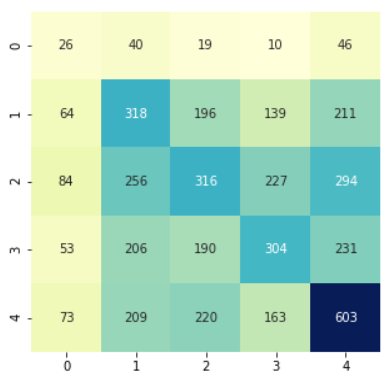
\includegraphics[scale=0.8]{confusionmatrix.png}
	\caption{Матрица ошибок модели SGDclassifier}\label{text:confusion}
\end{figure}

Также на рисунках \ref{text:words0} и \ref{text:words1} приведены токены, которые сыграли наибольшую роль при принятии решения, отнести питомца к 0 или 1 классу. Графики для оставшихся классов приведены в приложении.

\begin{figure}[H]
	\centering
	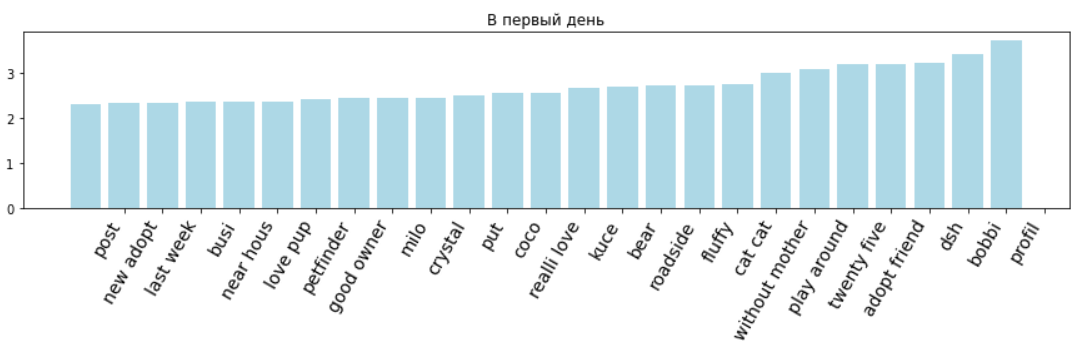
\includegraphics[scale=0.6]{words0.png}
	\caption{Важность слов для 0 класса}\label{text:words0}
\end{figure}

Как видно из рисунка \ref{text:words0}, по мнению модели, необходимо использовать слова и словосочетания “good owner”, “fluffy”, “without mother” и другие для того, чтобы питомца забрали в первый день, как его профиль попал на сайт.

Для того, чтобы животное забрали в первую неделю после того, как его профиль попал на сайт, необходимо использовать слова и словосочетания “bring home”, “miss”, “friend playful”, “food toilet” и другие (рисунок \ref{text:words1}).


\begin{figure}[H]
	\centering
	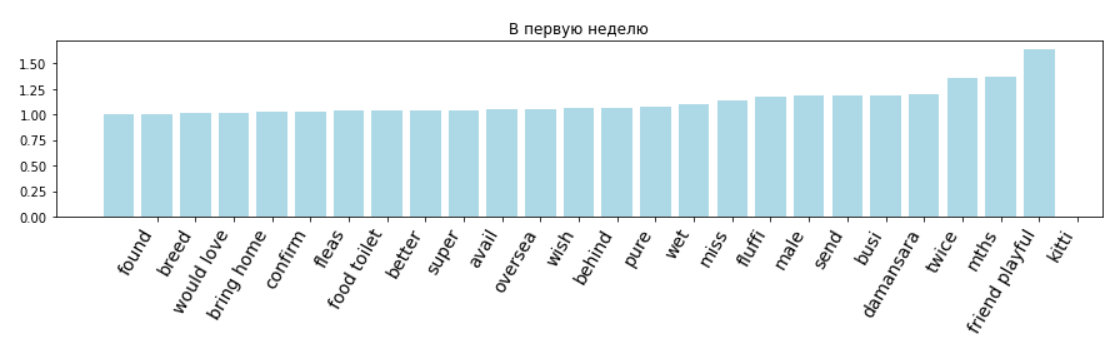
\includegraphics[scale=0.6]{words1.png}
	\caption{Важность слов для 1 класса}\label{text:words1}
\end{figure}

Таким образом, обработка естественного языка позволяет понять, какие слова необходимо использовать в описании для того, чтобы питомца как можно быстрее приняли в семью.


%=======================
\newpage
\section{Выбор датасета, модели и тестирование на Kaggle}

Модели, построенные на основе текстовых признаков, гораздо лучше отделяют нулевой класс от остальных. Поэтому, если необходимо определить как можно больше экземпляров 0 класса, то лучше использовать именно эти модели.
Но главная цель задачи на Kaggle [1] — получить как можно лучшее значение метрики. Поэтому необходимо использовать датасеты, содержащие не только текстовые признаки. 

Самое лучшее качество моделей показали датасеты, в которых часть выбросов в переменных Fee и Quantity были заменены выборочным значением. Замена переменной, оценивающей значение исходной, во всех 4 моделях получила худшее значение, чем замена выборочным. 

Также лучшее качество было на датасетах, в которых были применены методы шкалирования и кодирования переменных. Target Encoding и One Hot Encoding показали примерно одинаковые результаты, но выбор был сделан в пользу Target Encoding, так как он не расширяет пространство признаков и, следовательно, обучение на таком датасете происходит быстрее.

Среди моделей наилучшее качество показали ансамблевые алгоритмы. Случайный лес и Градиентный бустинг достигли качества метрики 0.42 на тестовой выборке, которая была получена из train\_test\_split.

При проверке качества на тестовом датасете test.csv на Kaggle модель градиентного бустинга (XGBoost) показала чуть лучшие результаты по сравнению с моделью случайного леса. 0.27 против 0.26 (рис. \ref{kaggle:result}). 

\begin{figure}[H]
	\centering
	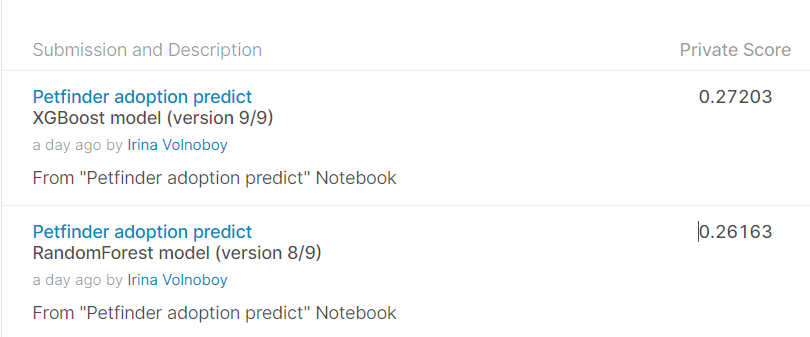
\includegraphics[scale=0.6]{kagglescore.png}
	\caption{Качество на тестовом датасете test.csv на Kaggle}\label{kaggle:result}
\end{figure}

Также возможно посмотреть, какие признаки внесли наибольший вклад в принятие решения. 

\begin{figure}[H]
	\centering
	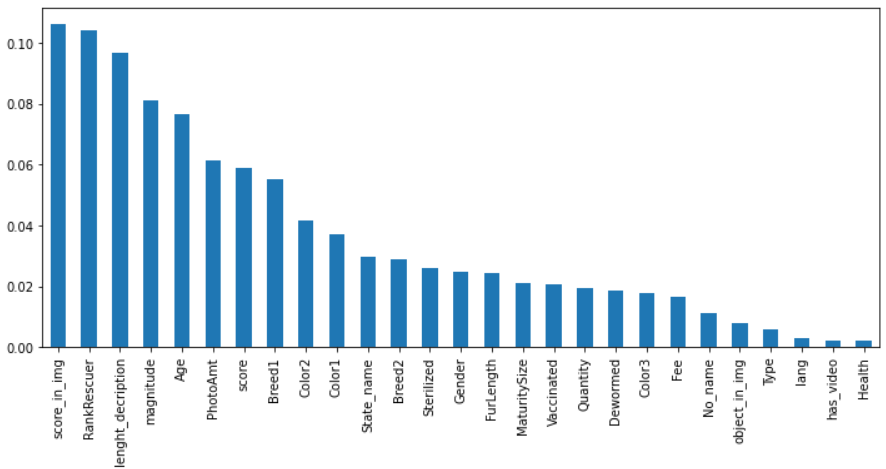
\includegraphics[scale=0.7]{featuresrfc.png}
	\caption{Важность признаков для модели RandomForestClassifier}\label{kaggle:rfc}
\end{figure}

Для модели случайного леса наиболее важными признаками оказались точность, с которой модель Google Vision определила объект на изображении, ранг человека, который создал профиль питомца, длина описания, а также его эмоциональная окраска (рисунок \ref{kaggle:rfc}).

Модель градиентного бустинга принимала решение, основываясь в основном на языке, на котором написано описание, возрасте питомца, ранге человека, на том, стерилизовано ли животное, а также на породе (см. рис. \ref{kaggle:boost}).


\begin{figure}[H]
	\centering
	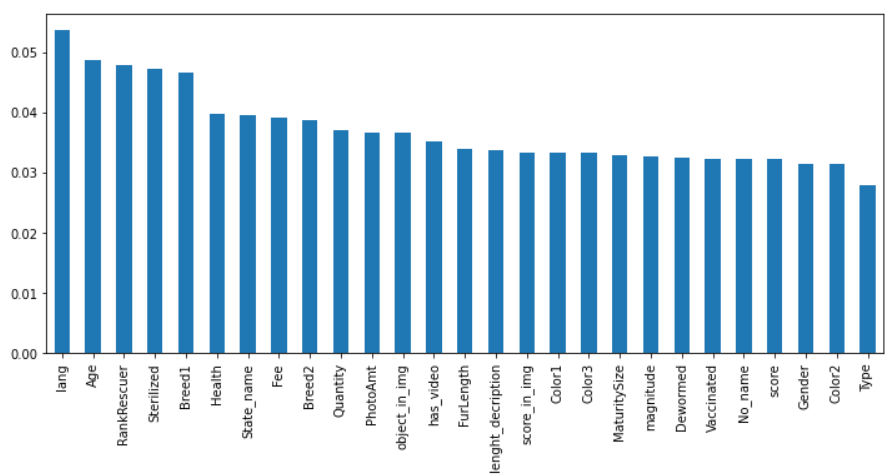
\includegraphics[scale=0.7]{featuresboost.png}
	\caption{Важность признаков для модели XGBoost}\label{kaggle:boost}
\end{figure}


%=======================
\newpage
\addcontentsline{toc}{section}{Заключение}
\section*{Заключение}

\textcolor{red}{После постановки задачи}

Результатом работы стали разработанные компоненты приложения для анализа онлайн-профиля животного \cite{lib:result}.



%=======================
\newpage

\addcontentsline{toc}{section}{Литература}
\renewcommand{\refname}{\centering \textbf{Литература}}

\begin{thebibliography}{0}
\bibitem{lib:taskkaggle}
Задача с Kaggle --- URL: https://www.kaggle.com/c/petfinder-adoption-prediction (дата обр. 12.05.2021)

\bibitem{lib:obz1}
M. Amrane, S. Oukid, I. Gagaoua, T. Ensari, ``Breast Cancer Classification Using Machine Learning Int. Conf. on Electric Electronics'', Computer Science Biomedical Engineering's Meeting, April 18--19, 2018.

\bibitem{lib:obz2}
Karan Bhatia, Shikhar Arora and Ravi Tomar, ``Diagnosis of Diabetic Retinopathy Using Machine Learning Classification Algorithm'', 2nd International Conference on Next Generation Computing Technologies (NGCT), 2016.

\bibitem{lib:obz3}
Kaylee Zhang, Sherine Zhang. PetFinder Challenge: Predicting Pet Adoption Speed --- URL: http://cs229.stanford.edu/proj2019spr/report/55.pdf 

\bibitem{lib:missingdata}
Boyan Angelov. Working with Missing Data in Machine Learning  [Электронный ресурс] --- URL:  https://towardsdatascience.com/working-with-missing-data-in-machine-learning-9c0a430df4ce

\bibitem{lib:outlier}
Mayank Tripathi. Knowing all about Outliers in Machine Learning  [Электронный ресурс] --- URL:  https://datascience.foundation/sciencewhitepaper/knowing-all-about-outliers-in-machine-learning

\bibitem{lib:outlier2}
Will Badr. 5 Ways to Detect Outliers/Anomalies that every Data Scientist Should Know (Python Code) [Электронный ресурс] --- URL: https://towardsdatascience.com/5-ways-to-detect-outliers-that-every-data-scientist-should-know-python-code-70a54335a623

\bibitem{lib:googlelang}
Документация по Google’s Natural Language API [Электронный ресурс] --- URL:  https://cloud.google.com/natural-language\#section-1 

\bibitem{lib:encode}
Jeff Hale. Smarter Ways to Encode Categorical Data for Machine Learning  [Электронный ресурс] --- URL:  https://towardsdatascience.com/smarter-ways-to-encode-categorical-data-for-machine-learning-part-1-of-3-6dca2f71b159 

\bibitem{lib:encoding}
Svideloc. Target Encoding Vs. One-hot Encoding with Simple Examples  [Электронный ресурс] --- URL:  https://medium.com/analytics-vidhya/target-encoding-vs-one-hot-encoding-with-simple-examples-276a7e7b3e64

\bibitem{lib:tarencode}
Konstantin Klepikov. Подготовка данных: кодирование категориальных признаков --- URL: https://konstantinklepikov.github.io/2019/10/28/data-preprocessing-category-encoders.html

\bibitem{lib:standardize}
Jeff Hale. Scale, Standardize, or Normalize with Scikit-Learn [Электронный ресурс] --- URL:  https://towardsdatascience.com/scale-standardize-or-normalize-with-scikit-learn-6ccc7d176a02

\bibitem{lib:sklearnstandard}
Документация библиотеки sklearn по функции StandardScaler  [Электронный ресурс] --- URL:  https://scikit-learn.org/stable/modules/generated/sklearn.preprocessing.StandardScaler.html 

\bibitem{lib:kappa1}
Aman Arora. Quadratic Kappa Metric explained in 5 simple steps  [Электронный ресурс] --- URL:  https://www.kaggle.com/aroraaman/quadratic-kappa-metric-explained-in-5-simple-steps 

\bibitem{lib:kappa2}
Aditya Kumar. Kappa Coefficient for Dummies [Электронный ресурс] --- URL:  https://medium.com/x8-the-ai-community/kappa-coefficient-for-dummies-84d98b6f13ee

\bibitem{lib:trees}
Prashant Gupta. Decision Trees in Machine Learning [Электронный ресурс] --- URL:  https://towardsdatascience.com/decision-trees-in-machine-learning-641b9c4e8052

\bibitem{lib:logreg}
Логистическая регрессия [Электронный ресурс] --- URL:  http://www.machinelearning.ru/wiki/index.php?title=Логистическая\_регрессия 

\bibitem{lib:logreg2}
Khushnuma Grover. Advantages and Disadvantages of Logistic Regression [Электронный ресурс] --- URL:  https://iq.opengenus.org/advantages-and-disadvantages-of-logistic-regression/ 

\bibitem{lib:randomforest}
Сергей Штукатуров. Реализация и разбор алгоритма «случайный лес» на Python [Электронный ресурс] --- URL: https://tproger.ru/translations/python-random-forest-implementation/

\bibitem{lib:randomforest2}
Vradchenko. Открытый курс машинного обучения. Тема 5. Композиции: бэггинг, случайный лес [Электронный ресурс] --- URL: https://habr.com/ru/company/ods/blog/324402/ 

\bibitem{lib:gradboost}
Harshdeep Singh. Understanding Gradient Boosting Machines [Электронный ресурс] --- URL: https://towardsdatascience.com/understanding-gradient-boosting-machines-9be756fe76ab

\bibitem{lib:gradboost2}
Rajat Panchotia. Introduction to Gradient Boosting Classification [Электронный ресурс] --- URL: https://medium.com/analytics-vidhya/introduction-to-gradient-boosting-classification-da4e81f54d3

\bibitem{lib:stemlem}
Stemming and lemmatization [Электронный ресурс] --- URL: https://nlp.stanford.edu/IR-book/html/htmledition/stemming-and-lemmatization-1.html (дата обр. 26.04.2021)

\bibitem{lib:langproc}
Steven Bird, Ewan Klein, Edward Loper. Natural Language Processing with Python // O’Reilly Media, Inc. — 2009. — First Edition. — С. 107–108.

\bibitem{lib:vect}
Nick Komissarenko. 4 метода векторизации текстов [Электронный ресурс] --- URL: https://medium.com/@bigdataschool/4-метода-векторизации-текстов-f8ac90e4175a (дата обр. 26.04.2021)

\bibitem{lib:tfidf}
Статья на Википедии TF-IDF [Электронный ресурс] --- URL: https://ru.wikipedia.org/wiki/TF-IDF 

\bibitem{lib:regular}
LASSO и RIDGE регуляризации для линейной регрессии [Электронный ресурс] --- URL: https://craftappmobile.com/l1-vs-l2-regularization/

\bibitem{lib:result}
Программная реализация задачи предсказания класса принятия питомца в семью --- URL: https://github.com/ivolnoboi/petfinder\_AdoptionPredict


\end{thebibliography}



%=======================
\newpage

\addcontentsline{toc}{section}{Приложение}
\section*{Приложение}

\begin{figure}[H]
	\centering
	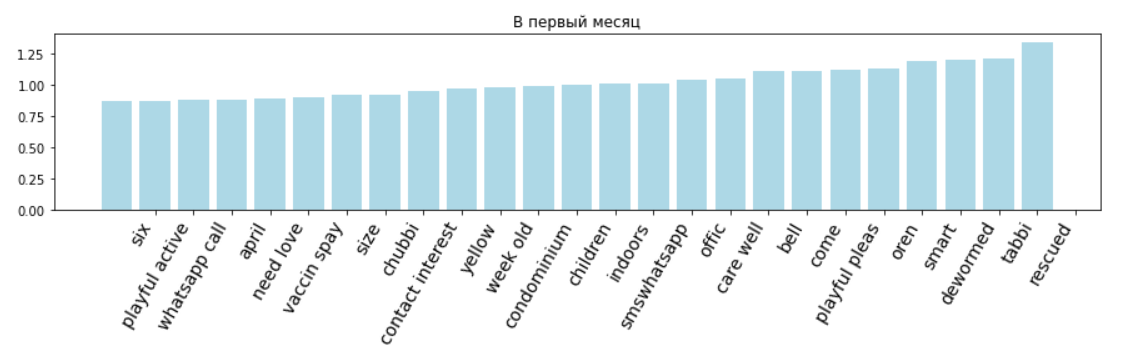
\includegraphics[scale=0.6]{words2.png}
	\caption{Важность слов для 2 класса}\label{text:words2}
\end{figure}

\begin{figure}[H]
	\centering
	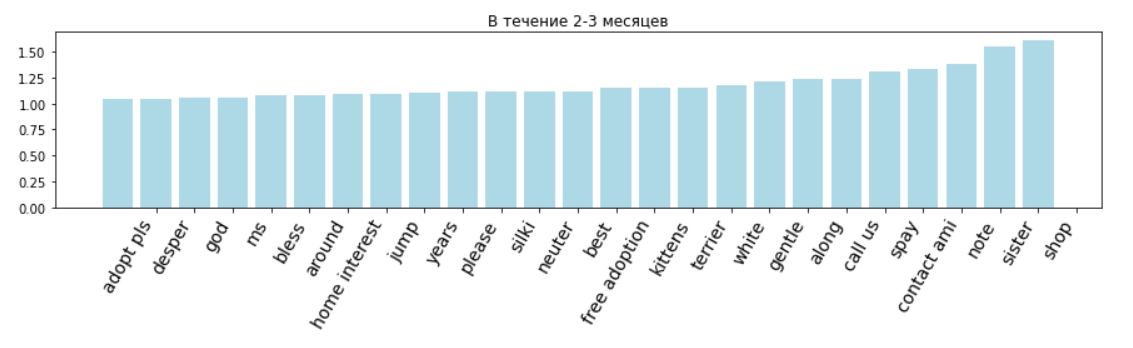
\includegraphics[scale=0.6]{words3.png}
	\caption{Важность слов для 3 класса}\label{text:words3}
\end{figure}

\begin{figure}[H]
	\centering
	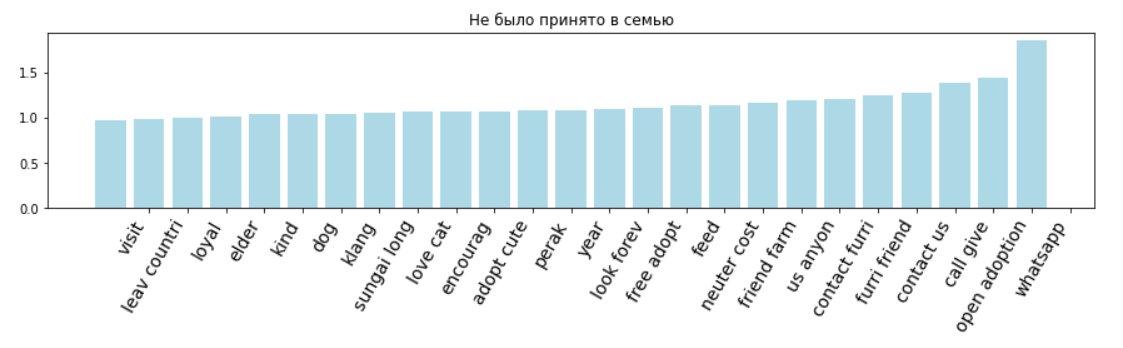
\includegraphics[scale=0.6]{words4.png}
	\caption{Важность слов для 4 класса}\label{text:words4}
\end{figure}



\end{document}
% ----------------------------------------------------------------


\lstset{ %
language=C++,                 % выбор языка для подсветки (здесь это С++)
basicstyle=\small\sffamily, % размер и начертание шрифта для подсветки кода
numbers=left,               % где поставить нумерацию строк (слева\справа)
numberstyle=\tiny,           % размер шрифта для номеров строк
stepnumber=1,                   % размер шага между двумя номерами строк
numbersep=5pt,                % как далеко отстоят номера строк от подсвечиваемого кода
backgroundcolor=\color{white}, % цвет фона подсветки - используем \usepackage{color}
showspaces=false,            % показывать или нет пробелы специальными отступами
showstringspaces=false,      % показывать или нет пробелы в строках
showtabs=false,             % показывать или нет табуляцию в строках
frame=single,              % рисовать рамку вокруг кода
tabsize=2,                 % размер табуляции по умолчанию равен 2 пробелам
captionpos=t,              % позиция заголовка вверху [t] или внизу [b]
breaklines=true,           % автоматически переносить строки (да\нет)
breakatwhitespace=false, % переносить строки только если есть пробел
escapeinside={\%*}{*)}   % если нужно добавить комментарии в коде
extendedchars=true,
commentstyle=\color{mygreen},    % comment style
stringstyle=\bf,
commentstyle=\ttfamily\itshape,
keepspaces=true % пробелы между русскими буквами
aboveskip=3mm,
belowskip=3mm

}


\renewcommand\NAT@bibsetnum[1]{\settowidth\labelwidth{\@biblabel{#1}}%
   \setlength{\leftmargin}{\bibindent}\addtolength{\leftmargin}{\dimexpr\labelwidth+\labelsep\relax}%
   \setlength{\itemindent}{-\bibindent+\fivecharsapprox}%
   \setlength{\listparindent}{\itemindent}
\setlength{\itemsep}{\bibsep}\setlength{\parsep}{\z@}%
   \ifNAT@openbib
     \addtolength{\leftmargin}{\bibindent}%
     \setlength{\itemindent}{-\bibindent}%
     \setlength{\listparindent}{\itemindent}%
     \setlength{\parsep}{0pt}%
   \fi
}
\renewcommand{\thesection}{\arabic{section}.}
\renewcommand{\thesubsection}{\arabic{section}.\arabic{subsection}.}
